
Przed rozpoczęciem pracy nad aplikacją stwierdzono możliwe zastosowania, które skorzystałyby z interfejsu graficznego do biblioteki przetwarzania obrazów.
Na ich podstawie zostały zdefiniowane wymagania funkcjonalne - dotyczące możliwości programu oraz wymagania niefunkcjonalne - mówiące o tym jak użytkownik będzie korzystał z projektu.

\subsection{Zastosowania}

\begin{itemize}
    \item \textbf{Tworzenie gotowych ciągów operacji:} Czasem potrzebne jest przetworzenie małej ilości obrazów, lub problem jest na tyle mało skomplikowany, że nie ma sensu szukać programisty, który stworzy dla nas program, ale bez wiedzy o programowaniu zrobienie tego w kodzie samodzielnie może być zbyt ciężkie. Program z interfejsem graficznym pozwoli na stworzenie procesów nawet przez osoby mniej techniczne.
    \item \textbf{Uczenie się:} Osoby chcące poznać techniki przetwarzania obrazów będą mogły w prosty sposób bez znajomości programowania zobaczyć na własne oczy działanie funkcji, ich interakcję ze sobą oraz łatwo dopasowywać ich parametry. 
    \item \textbf{Komunikacja:} Dzięki temu oprogramowaniu programista może łatwiej i efektywniej porozumieć się z osobami mniej zaznajomionymi z programowaniem i dużo szybciej wprowadzać zmiany w porównaniu z pisaniem kodu i jego kompilacją przy każdej zmianie.
\end{itemize}

\subsection{Analiza wymagań projektu}
Oprogramowanie opisane w tej pracy zostało nazwane \textbf{NoodleCV}. 
Następne podrozdziały przedstawią wymagania z jakimi trzeba było się zmierzyć w trakcie tworzenia aplikacji.

\subsubsection{Wymagania funkcjonalne}
Wymagania funkcjonalne?
\begin{itemize}
    \item Przetwarzanie obrazów
\end{itemize}

\subsubsection{Wymagania niefunkcjonalne}
Niefunkcjonalne wymagania?
\begin{itemize}
    \item Łatwość użytkowania
\end{itemize}

\subsection{Architektura aplikacji}


Projekt ten powstał w technologii Windows Presentation Foundation. 
Jedną z metod rozdzielenia widoku od logiki biznesowej w interfejsie tworzonym w WPF jest wzorzec MVVM (ang. \textit{Model-View-ViewModel}). 
Jego cel to jasny podział aplikacji na \textit{Model} - dane naszej aplikacji, ich interakcja ze sobą i implementacja mechanizmów działania oprogramowania. 
\textit{View} odpowiada tylko za wyświetlanie danych użytkownikowi oraz przyjmowanie jego interakcji jak kliknięcia czy wprowadzanie informacji. 
Za to klasy \textit{ViewModel} zajmują sie na połączeniu modelu i widoku konwertując obiekty z części biznesowej na dane które mają dotrzeć do użytkownika. 
Ich zadaniem jest też obsługa danych wprowadzanych przez interfejs aplikacji.

\subsubsection{Model}

\begin{figure}[H]
    \centering
    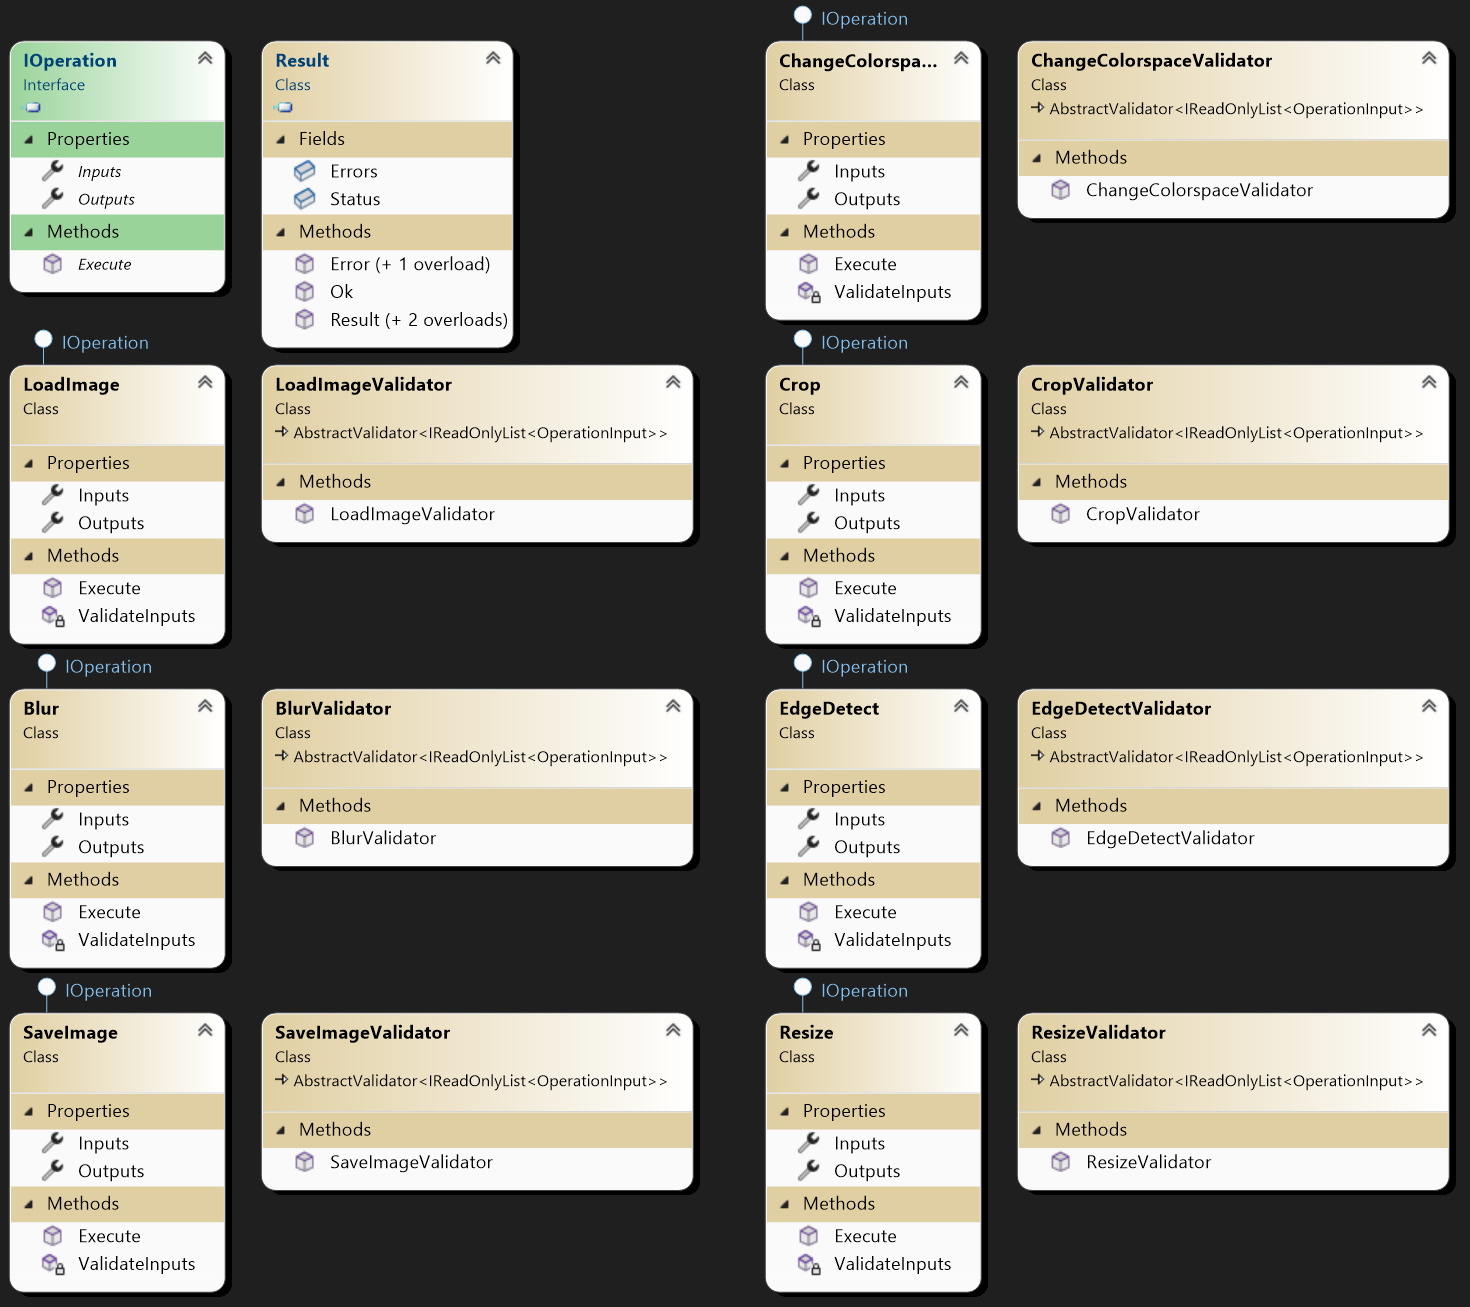
\includegraphics[width=1\linewidth]{images/Picture11.png}
    \caption{Diagram operacji. Opracowanie własne.}
    \label{fig:modelDiag}
\end{figure}

W NoodleCV warstwa \textit{Model} jest minimalna \autoref{fig:modelDiag}. 
Posiada interfejs IOperation odpowiadający za formę wszystkich implementacji operacji. 
Posiadają generyczna kolekcje wejść \textit{Inputs} oraz wyjść \textit{Outputs}.
Jedyna metoda zdefiniowana w nich to wykonanie operacji - zwraca ona obiekt \textit{Result}.
Informuje ona następne warstwy czy operacja się powiodła, jeżeli nie to dlaczego. 
Listę błędów otrzymujemy dzięki sprawdzeniu wejść za pomocą biblioteki Fluent Validation. 
Każda operacja wymaga swojego własnego walidatora danych i zapewnia tym bezpieczne działanie aplikacji - użytkownik nie powinien być w stanie doprowadzić programu do błędu złym parametrem operacji.

\begin{figure}[H]
    \centering
    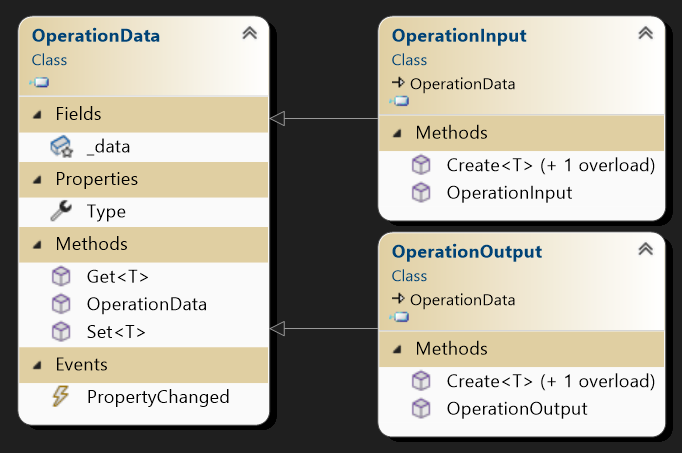
\includegraphics[width=0.6\linewidth]{images/Picture12.png}
    \caption{Diagram generycznych typów przechowujących dane operacji. Opracowanie własne.}
    \label{fig:input}
\end{figure}

Wejścia i wyjścia parametrów operacji mogą być w wielu różnych typach więc kolekcje przyjmujące te dane musiały być generyczne. 
Daje to dużo większą elastyczność ale może utrudnić implementację. 
Tworząc operacje i ich późniejsze \textit{ViewModel}'e trzeba zachować szczególną ostrożność. 
Przy tworzeniu nowych modeli zakładamy że obiekt w tym miejscu kolekcji będzie miał odpowiedni typ. 
Przy odczytywaniu danych z tej kolekcji nie ma informacji co to za klasa, należy poprawnie narzucić jej rodzaj inaczej napotkamy błąd i aplikacja wyłącza się.
Pomimo tych problemów warto korzystać z tej struktury ponieważ niektóre operacje przyjmują tylko ścieżkę do pliku w formie tekstu, inne mogą nie mieć żadnego wyjścia ale wszystkie pasują do jednego wspólnego interfejsu.

\subsubsection{View}

\begin{figure}[H]
    \centering
    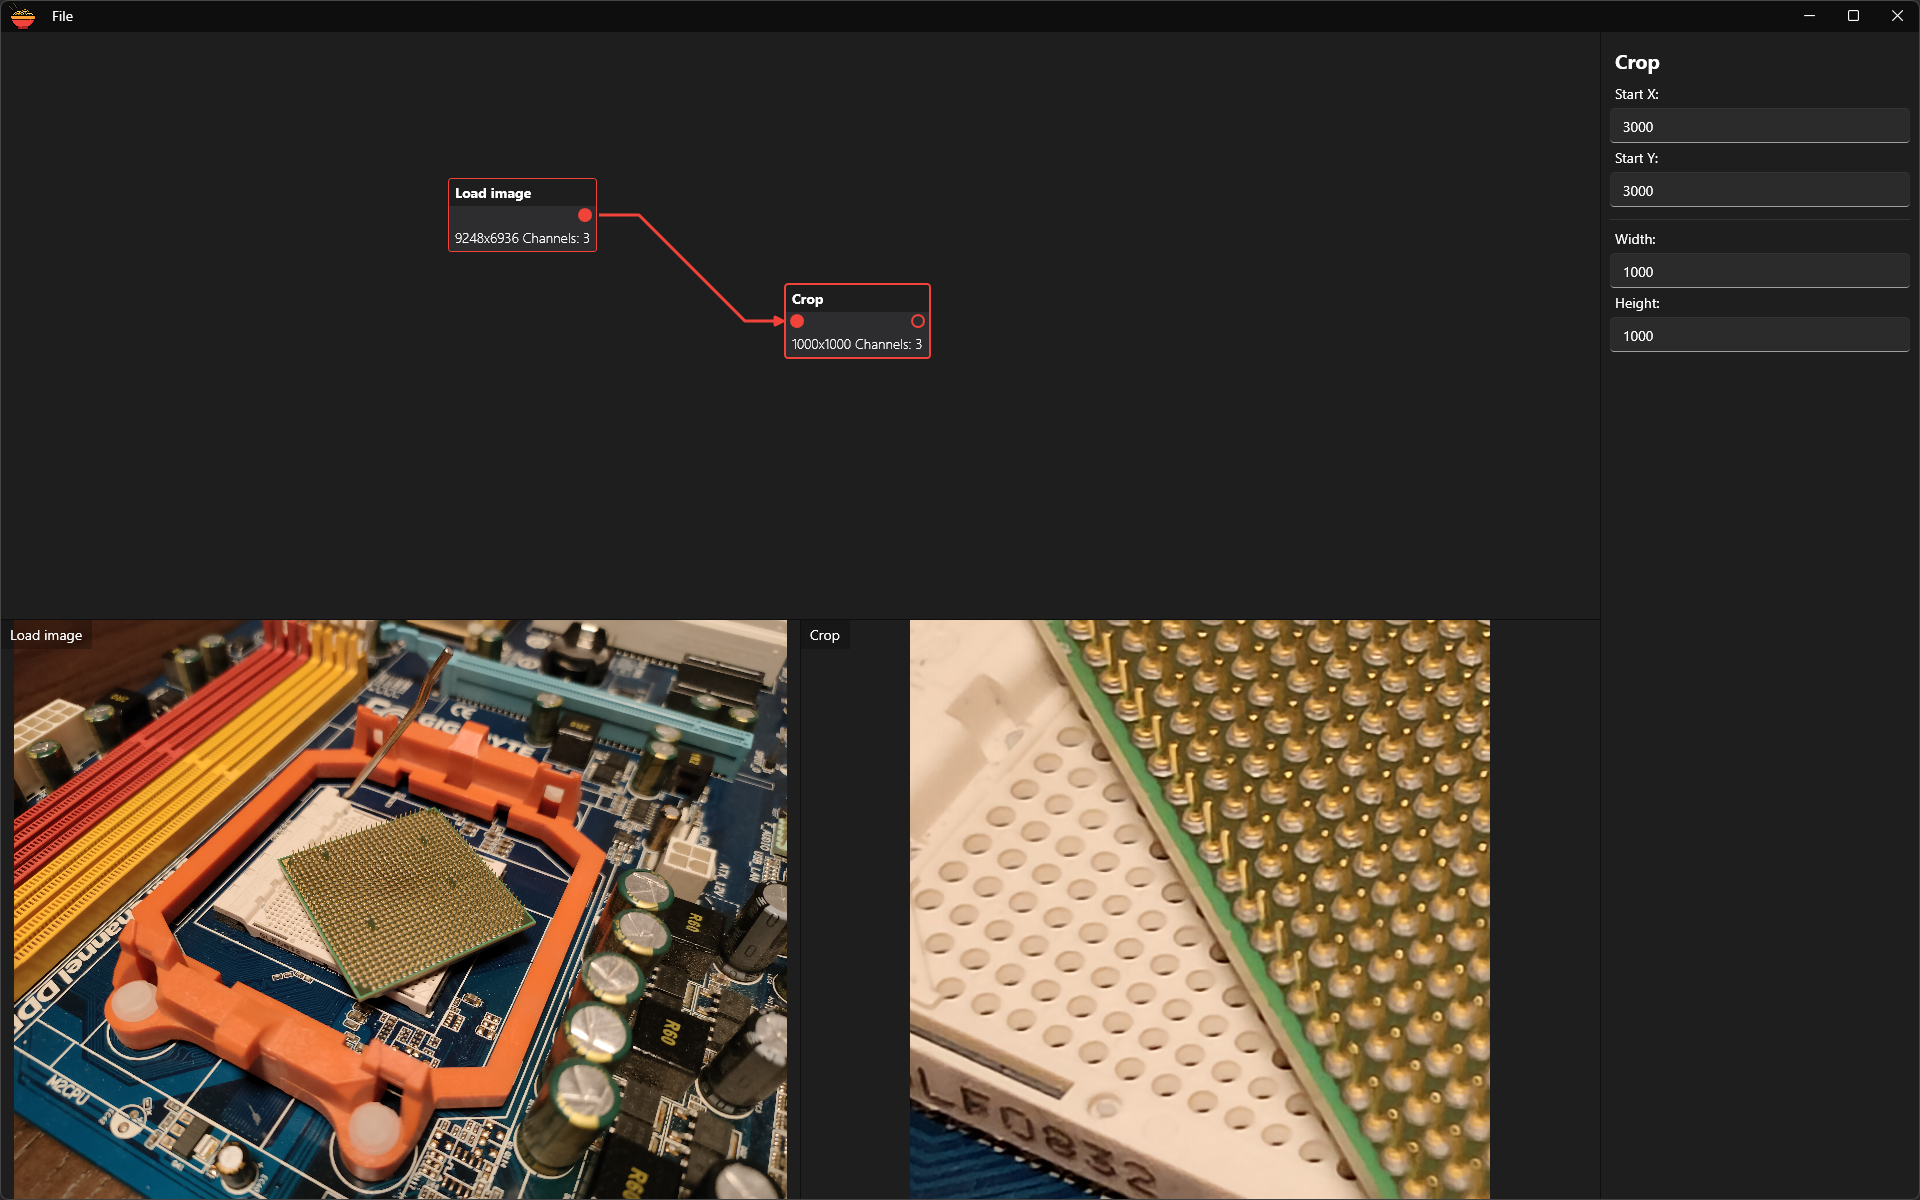
\includegraphics[width=1\linewidth]{images/Picture13.png}
    \caption{Główne okno aplikacji po starcie. Opracowanie własne.}
    \label{fig:window}
\end{figure}

Aplikacja posiada jedno okno \autoref{fig:window}. 
Użyta została klasa \textit{UiWindow} z biblioteki WPF UI pozwalająca łatwo zmodyfikować górny pasek by pasował do nowoczesnych systemów operacyjnych. 

\begin{figure}[H]
    \centering
    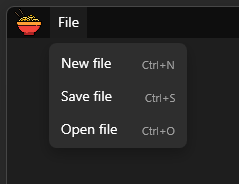
\includegraphics[width=0.6\linewidth]{images/Picture14.png}
    \caption{Menu aplikacji. Opracowanie własne.}
    \label{fig:mainmenu}
\end{figure}

Menu pozwala na zapisywanie odczytywanie lub czyszczenie stanu aplikacji. 
Opcje te są też przypisane znanym skrótom klawiszowym w celu ułatwienia ich używania.

Zawartość okna znajduje się w osobnym widoku edytora. Jest on podzielony na 3 główne elementy. Edytor \autoref{fig:editor} gdzie dodaje się nowe operacje, podgląd \autoref{fig:preview} gdzie pojawiają się wyniki operacji i panel od modyfikacji parametru \autoref{fig:params}.

\begin{figure}[H]
    \centering
    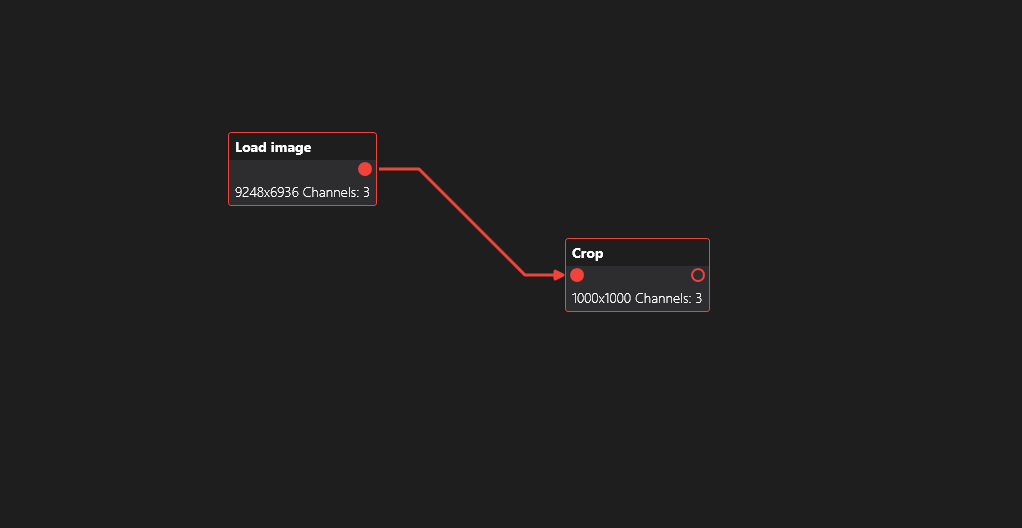
\includegraphics[width=1\linewidth]{images/Picture15.png}
    \caption{Widok edytora. Opracowanie własne.}
    \label{fig:editor}
\end{figure}

\begin{figure}[H]
    \centering
    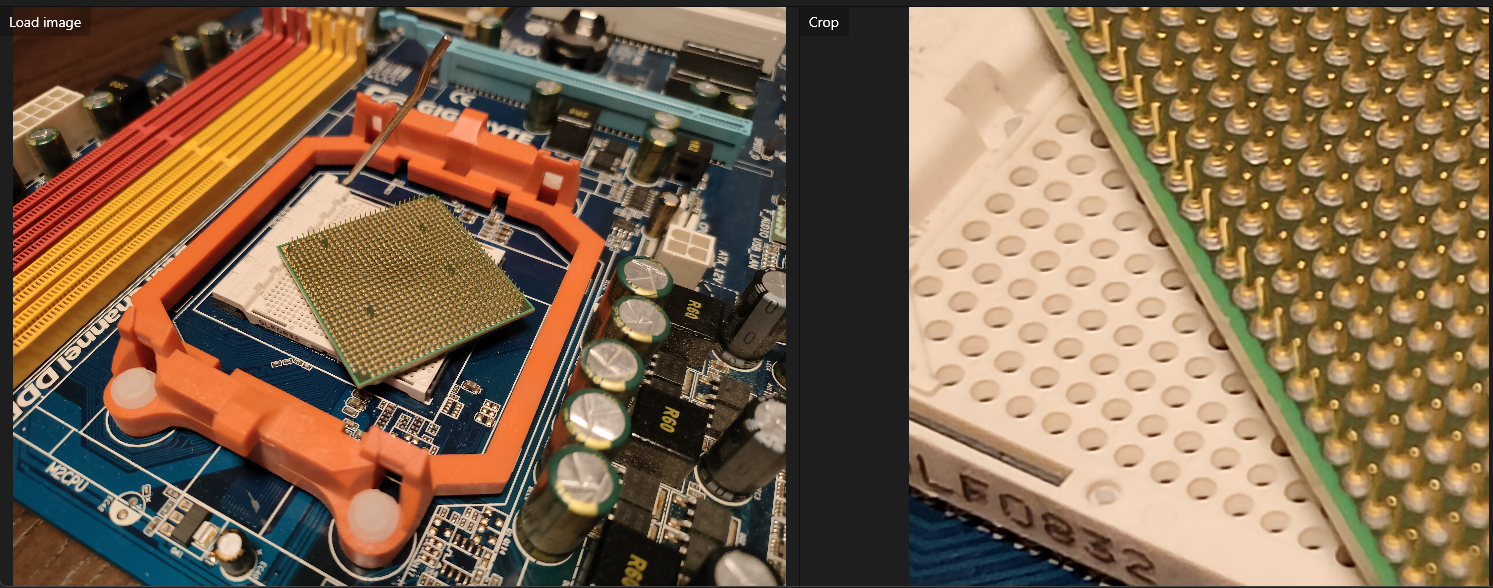
\includegraphics[width=1\linewidth]{images/Picture16.png}
    \caption{Podgląd wyników operacji. Opracowanie własne.}
    \label{fig:preview}
\end{figure}

\begin{figure}[H]
    \centering
    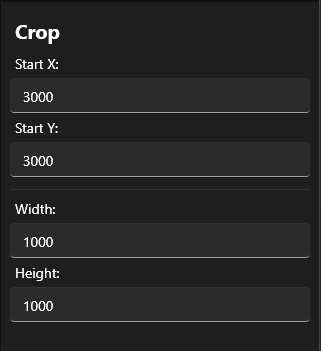
\includegraphics[width=0.6\linewidth]{images/Picture17.png}
    \caption{Edycja parametrów. Opracowanie własne.}
    \label{fig:params}
\end{figure}
\subsubsection{ViewModel}


\subsection{Zaimplementowane operacje}

Dla każdej operacji zostanie wczytany ten sam obraz i zamieszczone poniżej zrzuty ekranu będą prezentowały podgląd zdjęcia przed i po, a także panel z parametrami.
Zaimplementowano najpopularniejsze \cite{mostpop} metody, które pasowały do obecnych założeń projektu - operacja powinna przetwarzać obraz i zwracać obraz jako wynik.
\subsubsection{Blur}
\begin{figure}[H]
    \centering
    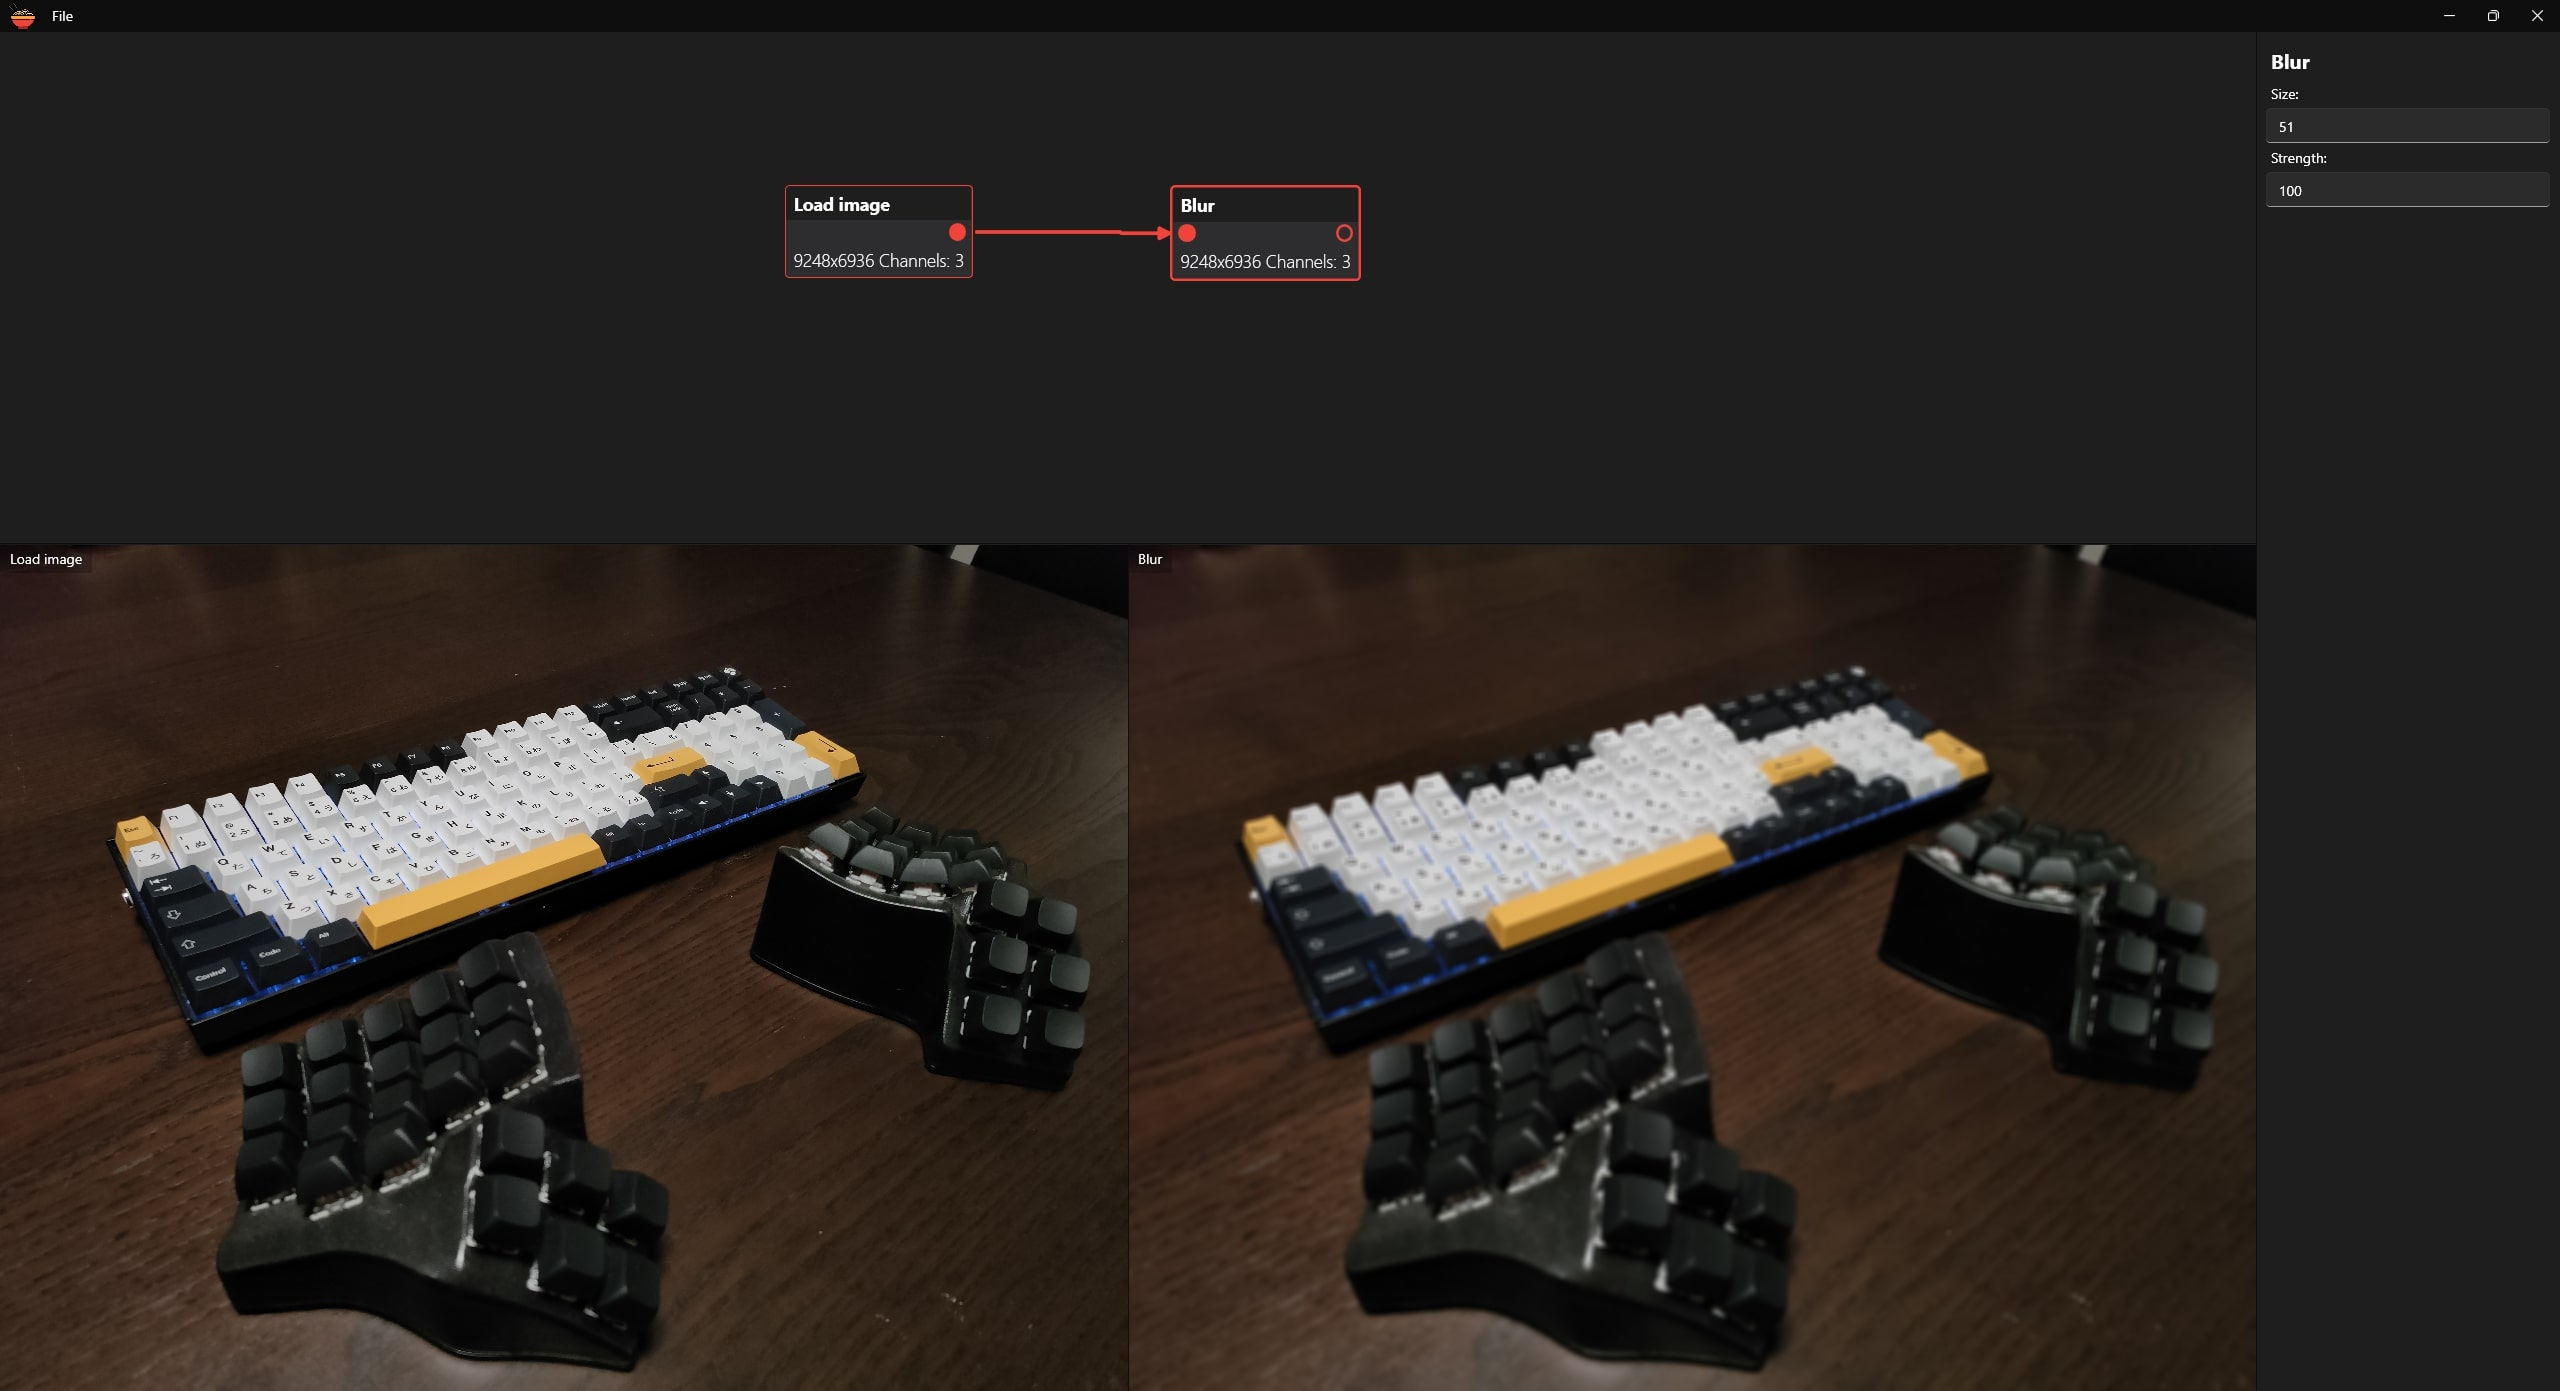
\includegraphics[width=1\linewidth]{images/Picture22.jpg}
    \caption{Operacja \textit{Blur}. Opracowanie własne.}
    \label{fig:blur}
\end{figure}

Zaimplementowana w oparciu o \textit{Gaussian Blur} \cite{gauss} (\autoref{fig:blur}). Parametr \textit{Size} musi być nieparzysty ponieważ opisuje on rozmiar maski na podstawie której wartość piksela jest uśredniana - potrzeby jest środek. \textit{Strength} opisuje natomiast odchylenie standardowe jakie będzie zastosowane przy przeprowadzaniu operacji.

\subsubsection{ChangeColorspace}

\begin{figure}[H]
    \centering
    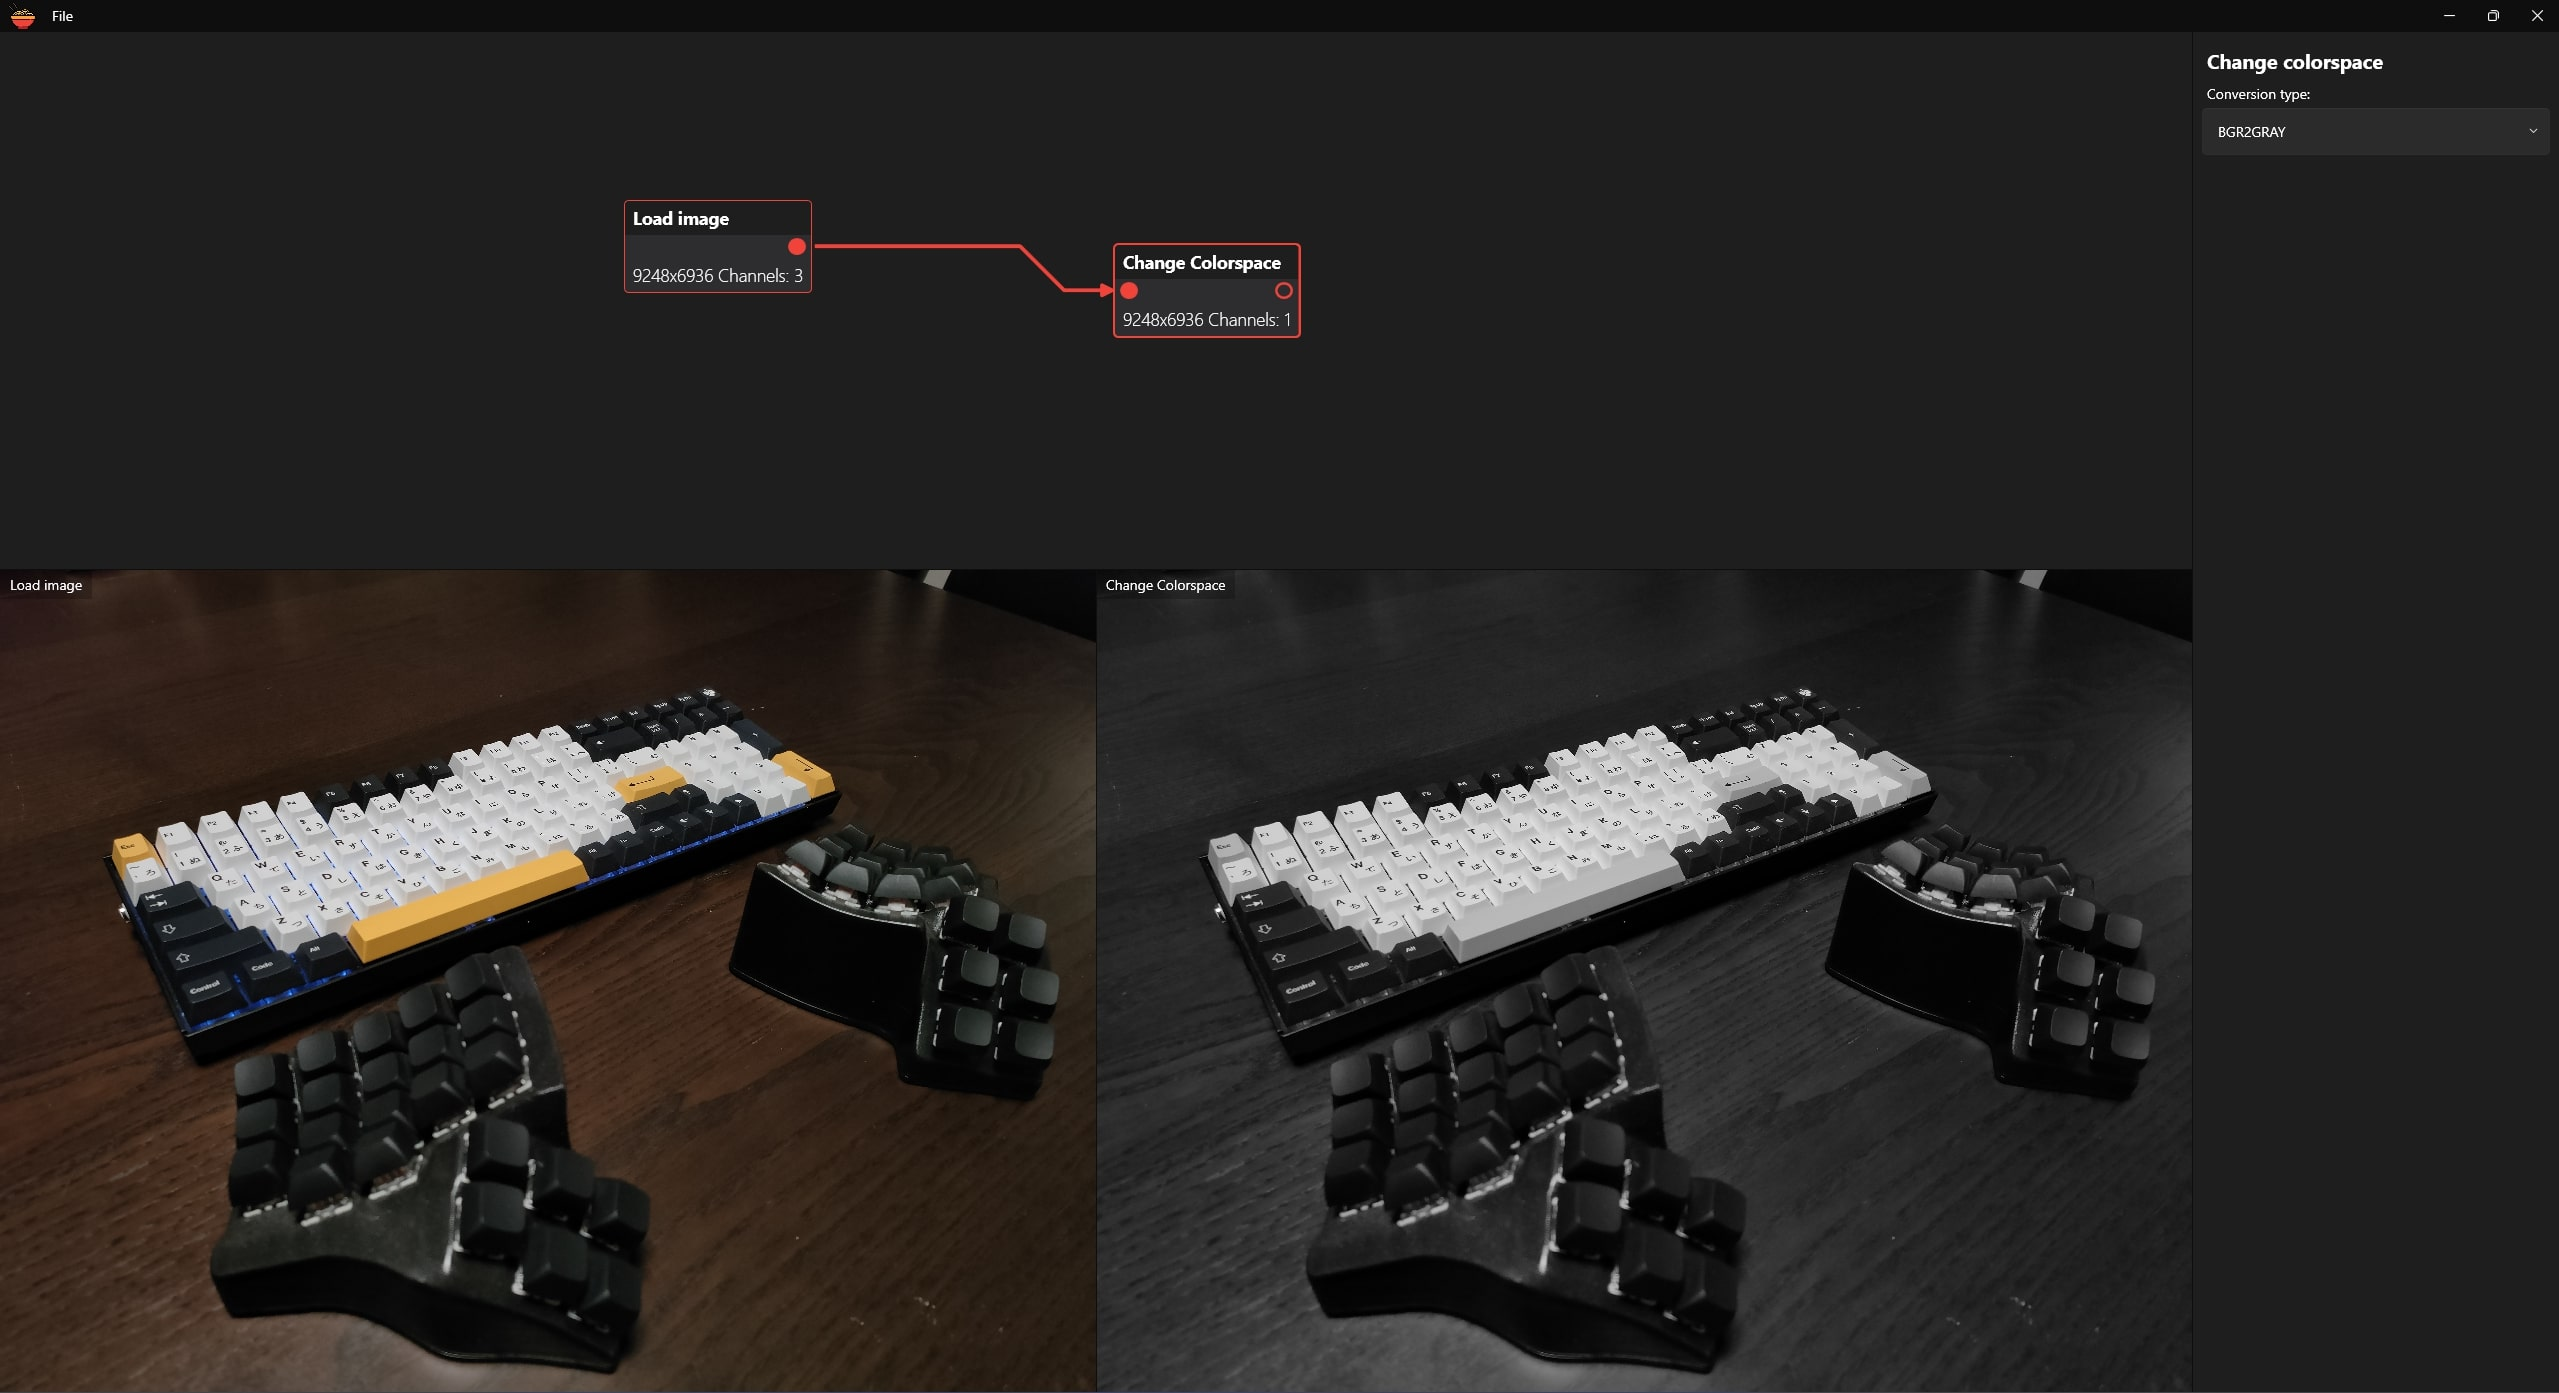
\includegraphics[width=1\linewidth]{images/Picture23.jpg}
    \caption{Operacja \textit{ChangeColorspace}. Opracowanie własne.}
    \label{fig:colorconv}
\end{figure}

Jest to funkcja \textit{CvtColor} \cite{cvtcol} (\autoref{fig:colorconv}). Konwertuje ona przestrzeń kolorów obrazu i dopasowuje ilość kanałów.
Jej jedynym parametrem jest kod z rodzajem konwersji np. \textit{BGR2GRAY} oznaczający przejście ze zwykłego kolorowego zdjęcia na biało-czarne.

\subsubsection{Crop}

\begin{figure}[H]
    \centering
    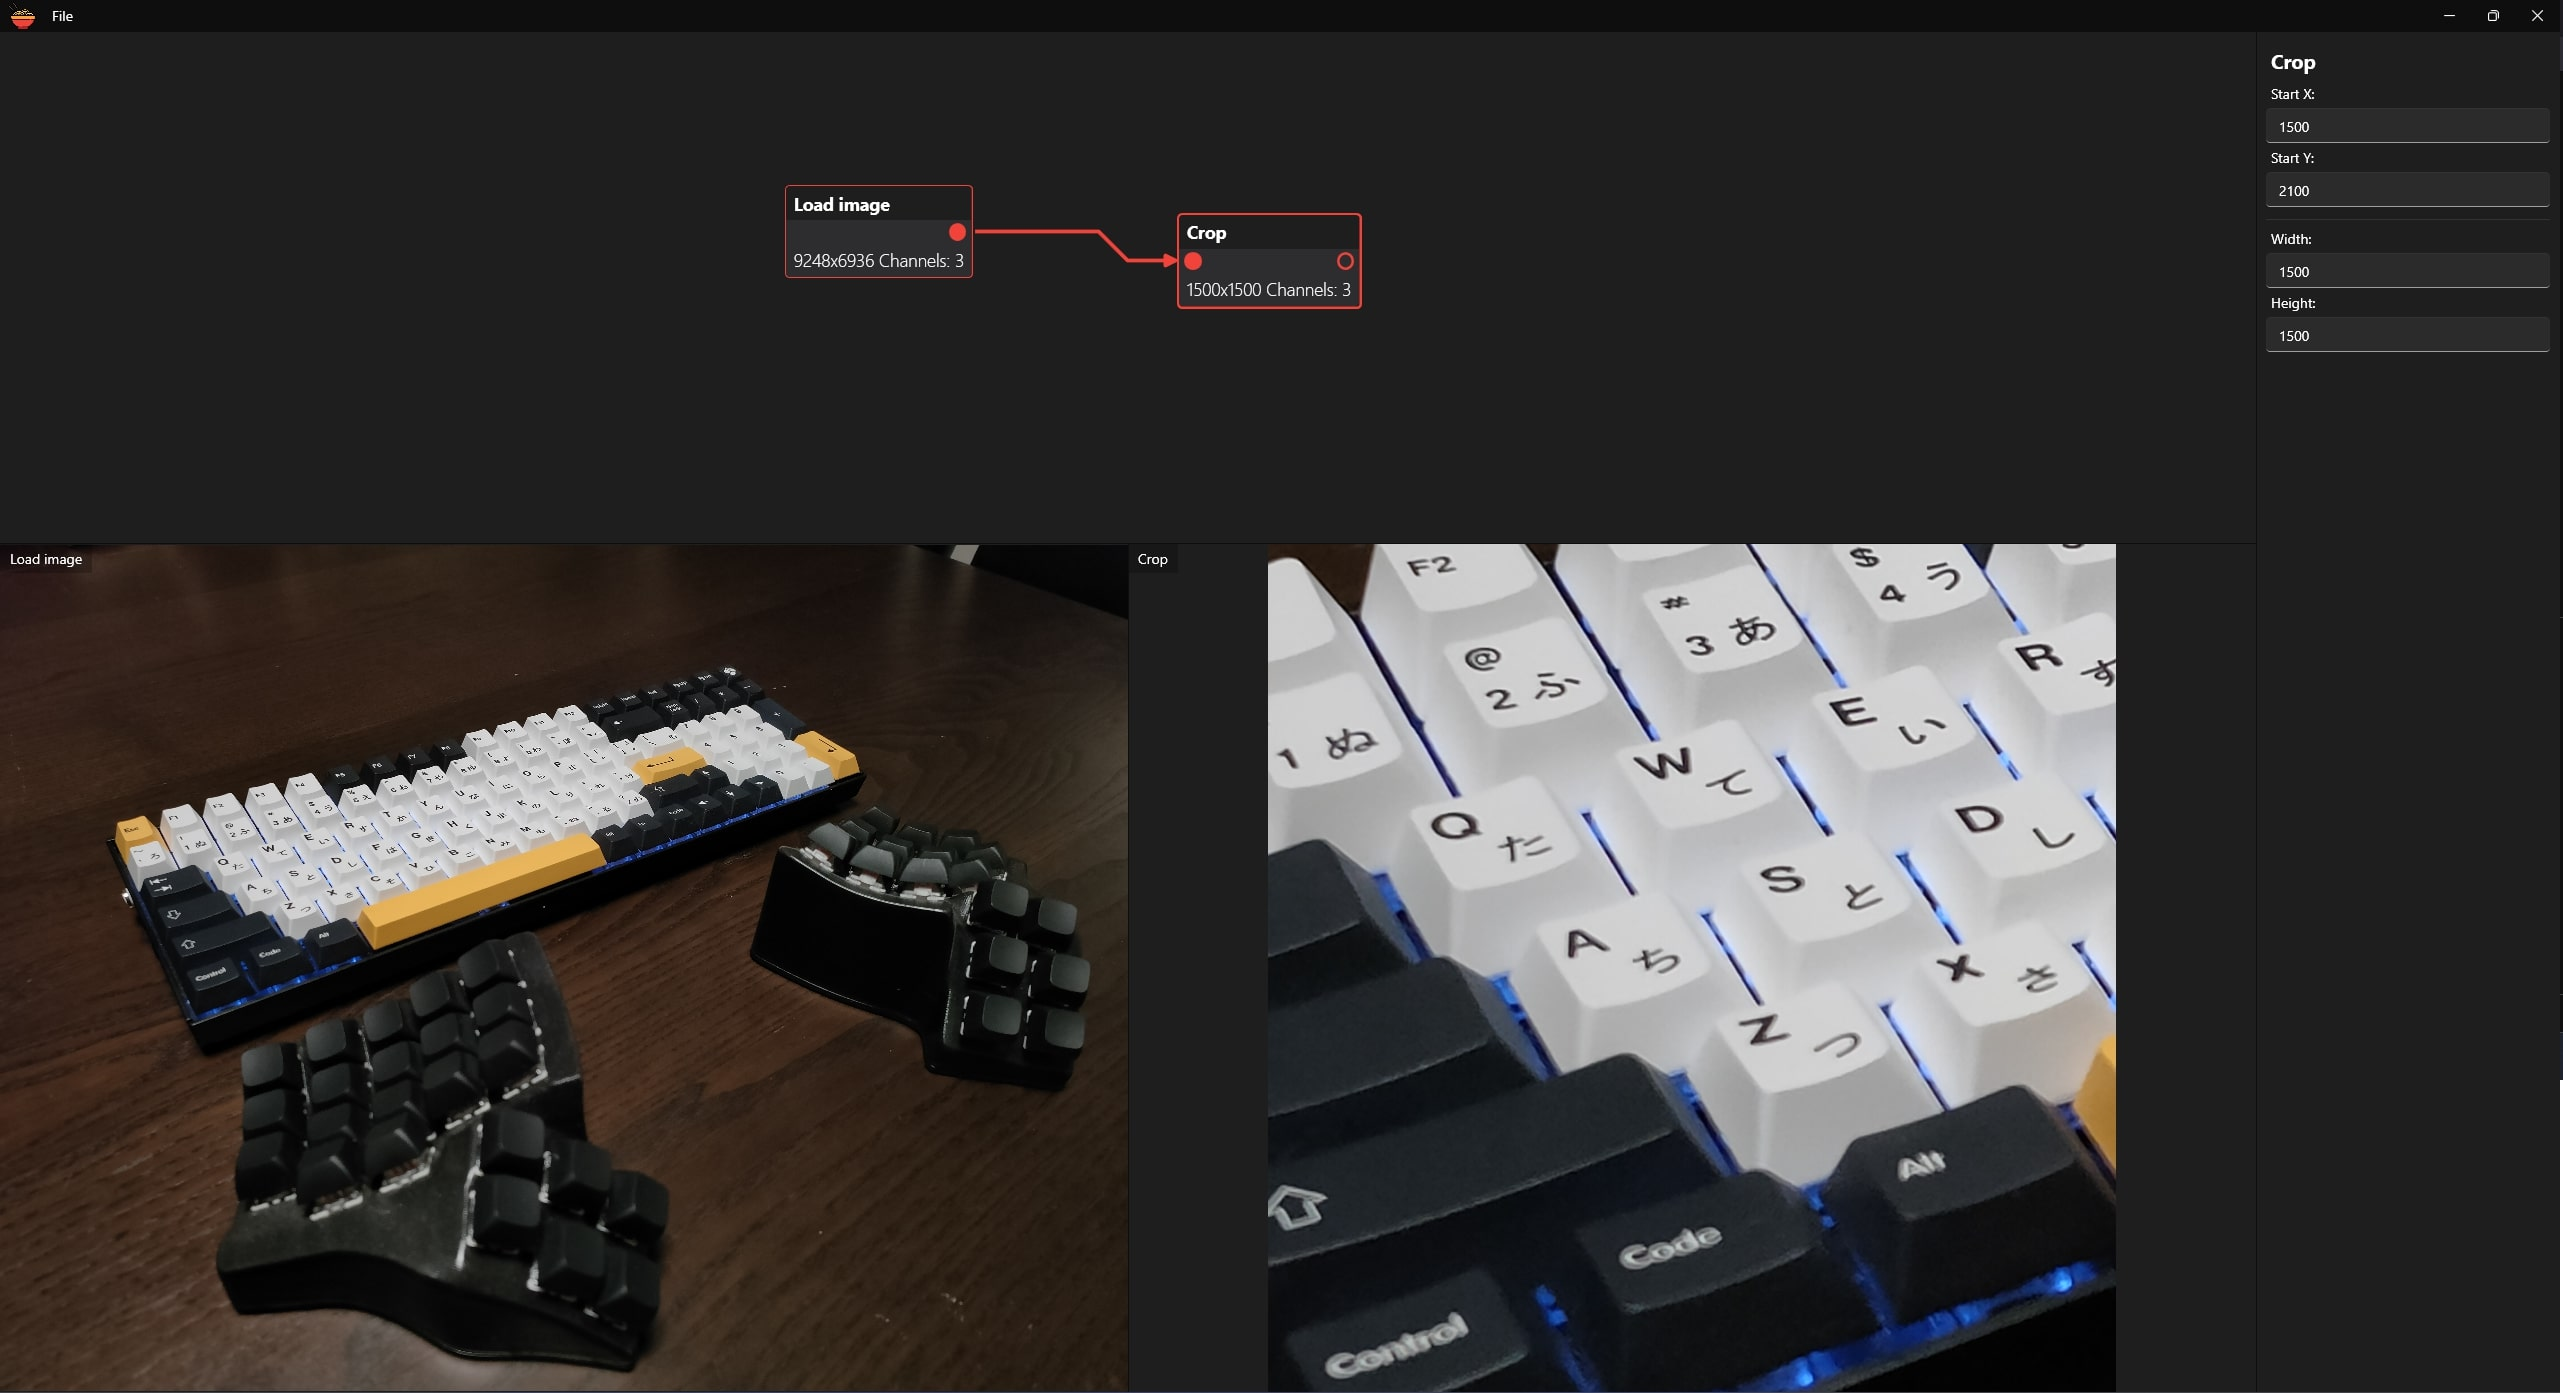
\includegraphics[width=1\linewidth]{images/Picture24.jpg}
    \caption{Operacja \textit{Crop}. Opracowanie własne.}
    \label{fig:crop}
\end{figure}

Operacja przycinania (ang. \textit{crop}) (\autoref{fig:crop}) jest realizowana poprzez wykorzystanie koordynatów początkowych, a także określenia wysokości i szerokości nowo tworzonego prostokąta. Po zdefiniowaniu tych czterech parametrów, użytkownik uzyskuje nowy obraz, którego wymiary odpowiadają podanym wartościom, a punkt początkowy określa jego położenie w ramach oryginalnego obrazu.

\subsubsection{EdgeDetect}

\begin{figure}[H]
    \centering
    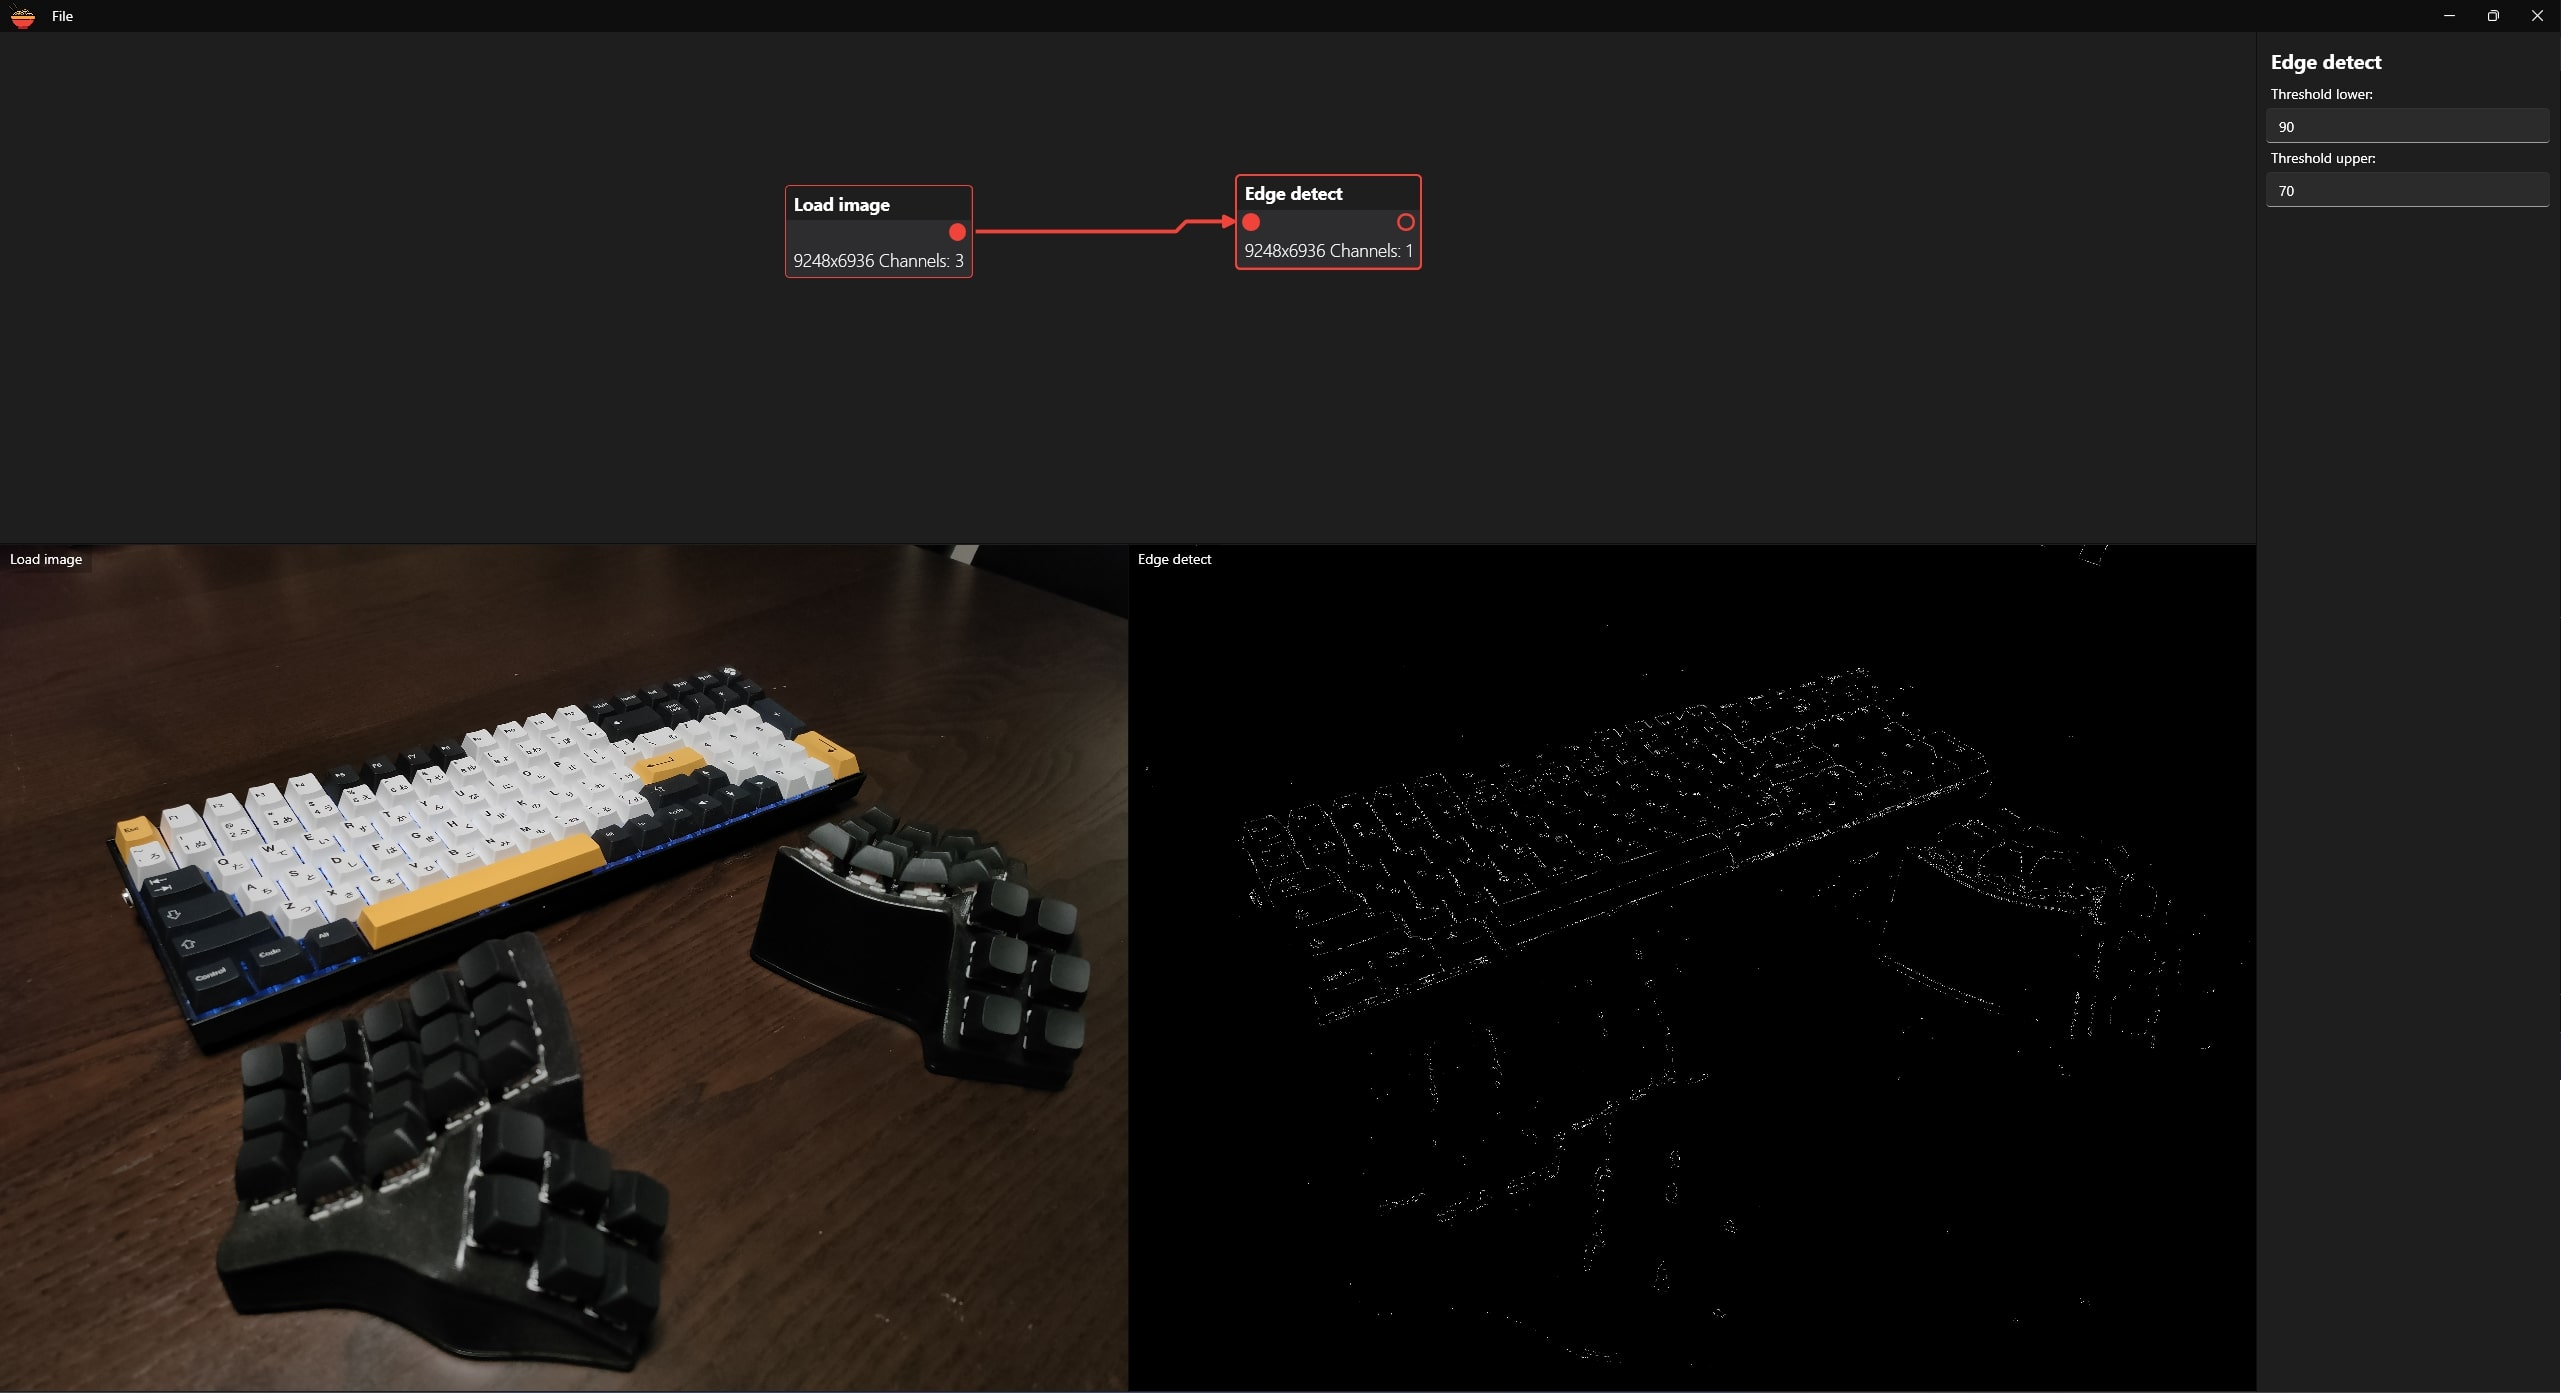
\includegraphics[width=1\linewidth]{images/Picture25.jpg}
    \caption{Operacja \textit{EdgeDetect}. Opracowanie własne.}
    \label{fig:edgeDetect}
\end{figure}  

Metoda \textit{Canny} \cite{canny} (\autoref{fig:edgeDetect}) to jeden z kilku dostępnych algorytmów wykrywania krawędzi. Jako parametry wejściowe należy podać niższy i wyższy próg akceptacji.
Jeżeli krawędź jest mało wyraźna zostaje odrzucona przez algorytm. 
Wartości powyżej drugiego parametru są uznawane za krawędź, a te które są pomiędzy zostają włączone do wyniku jako element łączący krawędzie jeżeli taki jest. 

\subsubsection{Resize}

\begin{figure}[H]
    \centering
    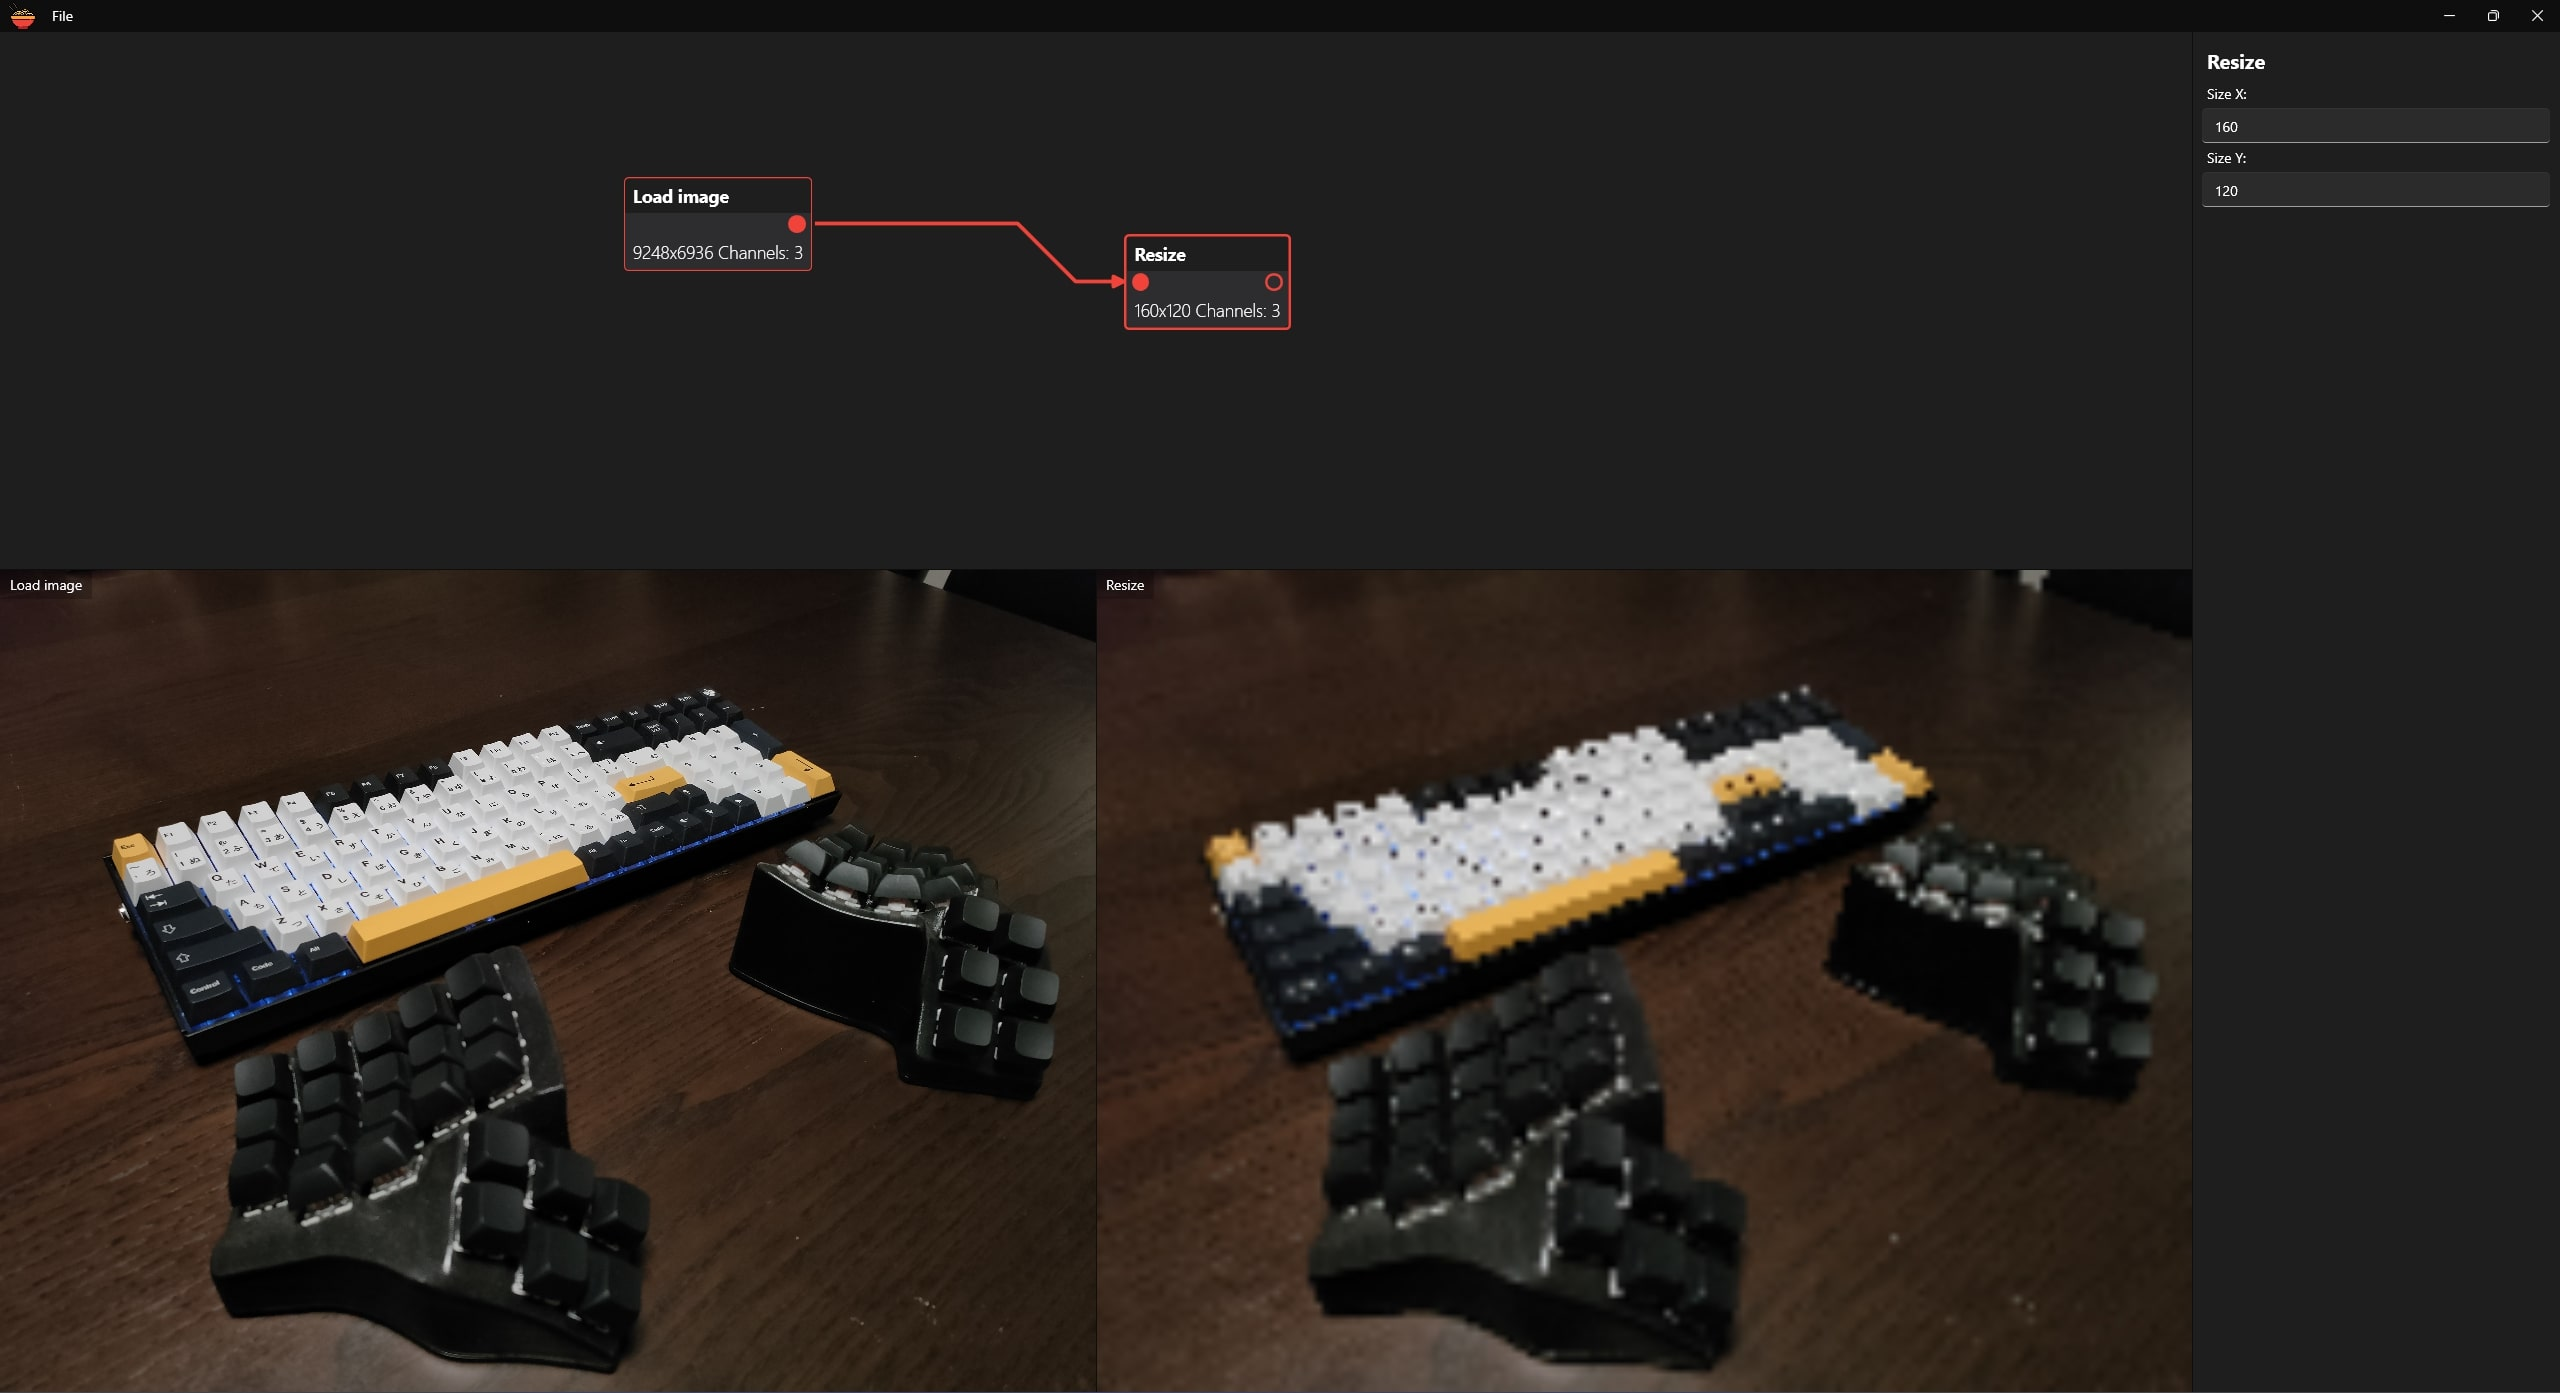
\includegraphics[width=1\linewidth]{images/Picture26.jpg}
    \caption{Operacja \textit{Resize}. Opracowanie własne.}
    \label{fig:resize}
\end{figure} 

\textit{Resize} (\autoref{fig:resize}) jest wykonywane przez metodę o tej samej nazwie z biblioteki OpenCV \cite{resize}. Po podaniu nowych wymiarów otrzymujemy obraz stworzony na podstawie oryginalnego ze zmienioną rozdzielczością.

\subsection{Przykładowe ciągi operacji}

\begin{figure}[H]
    \centering
    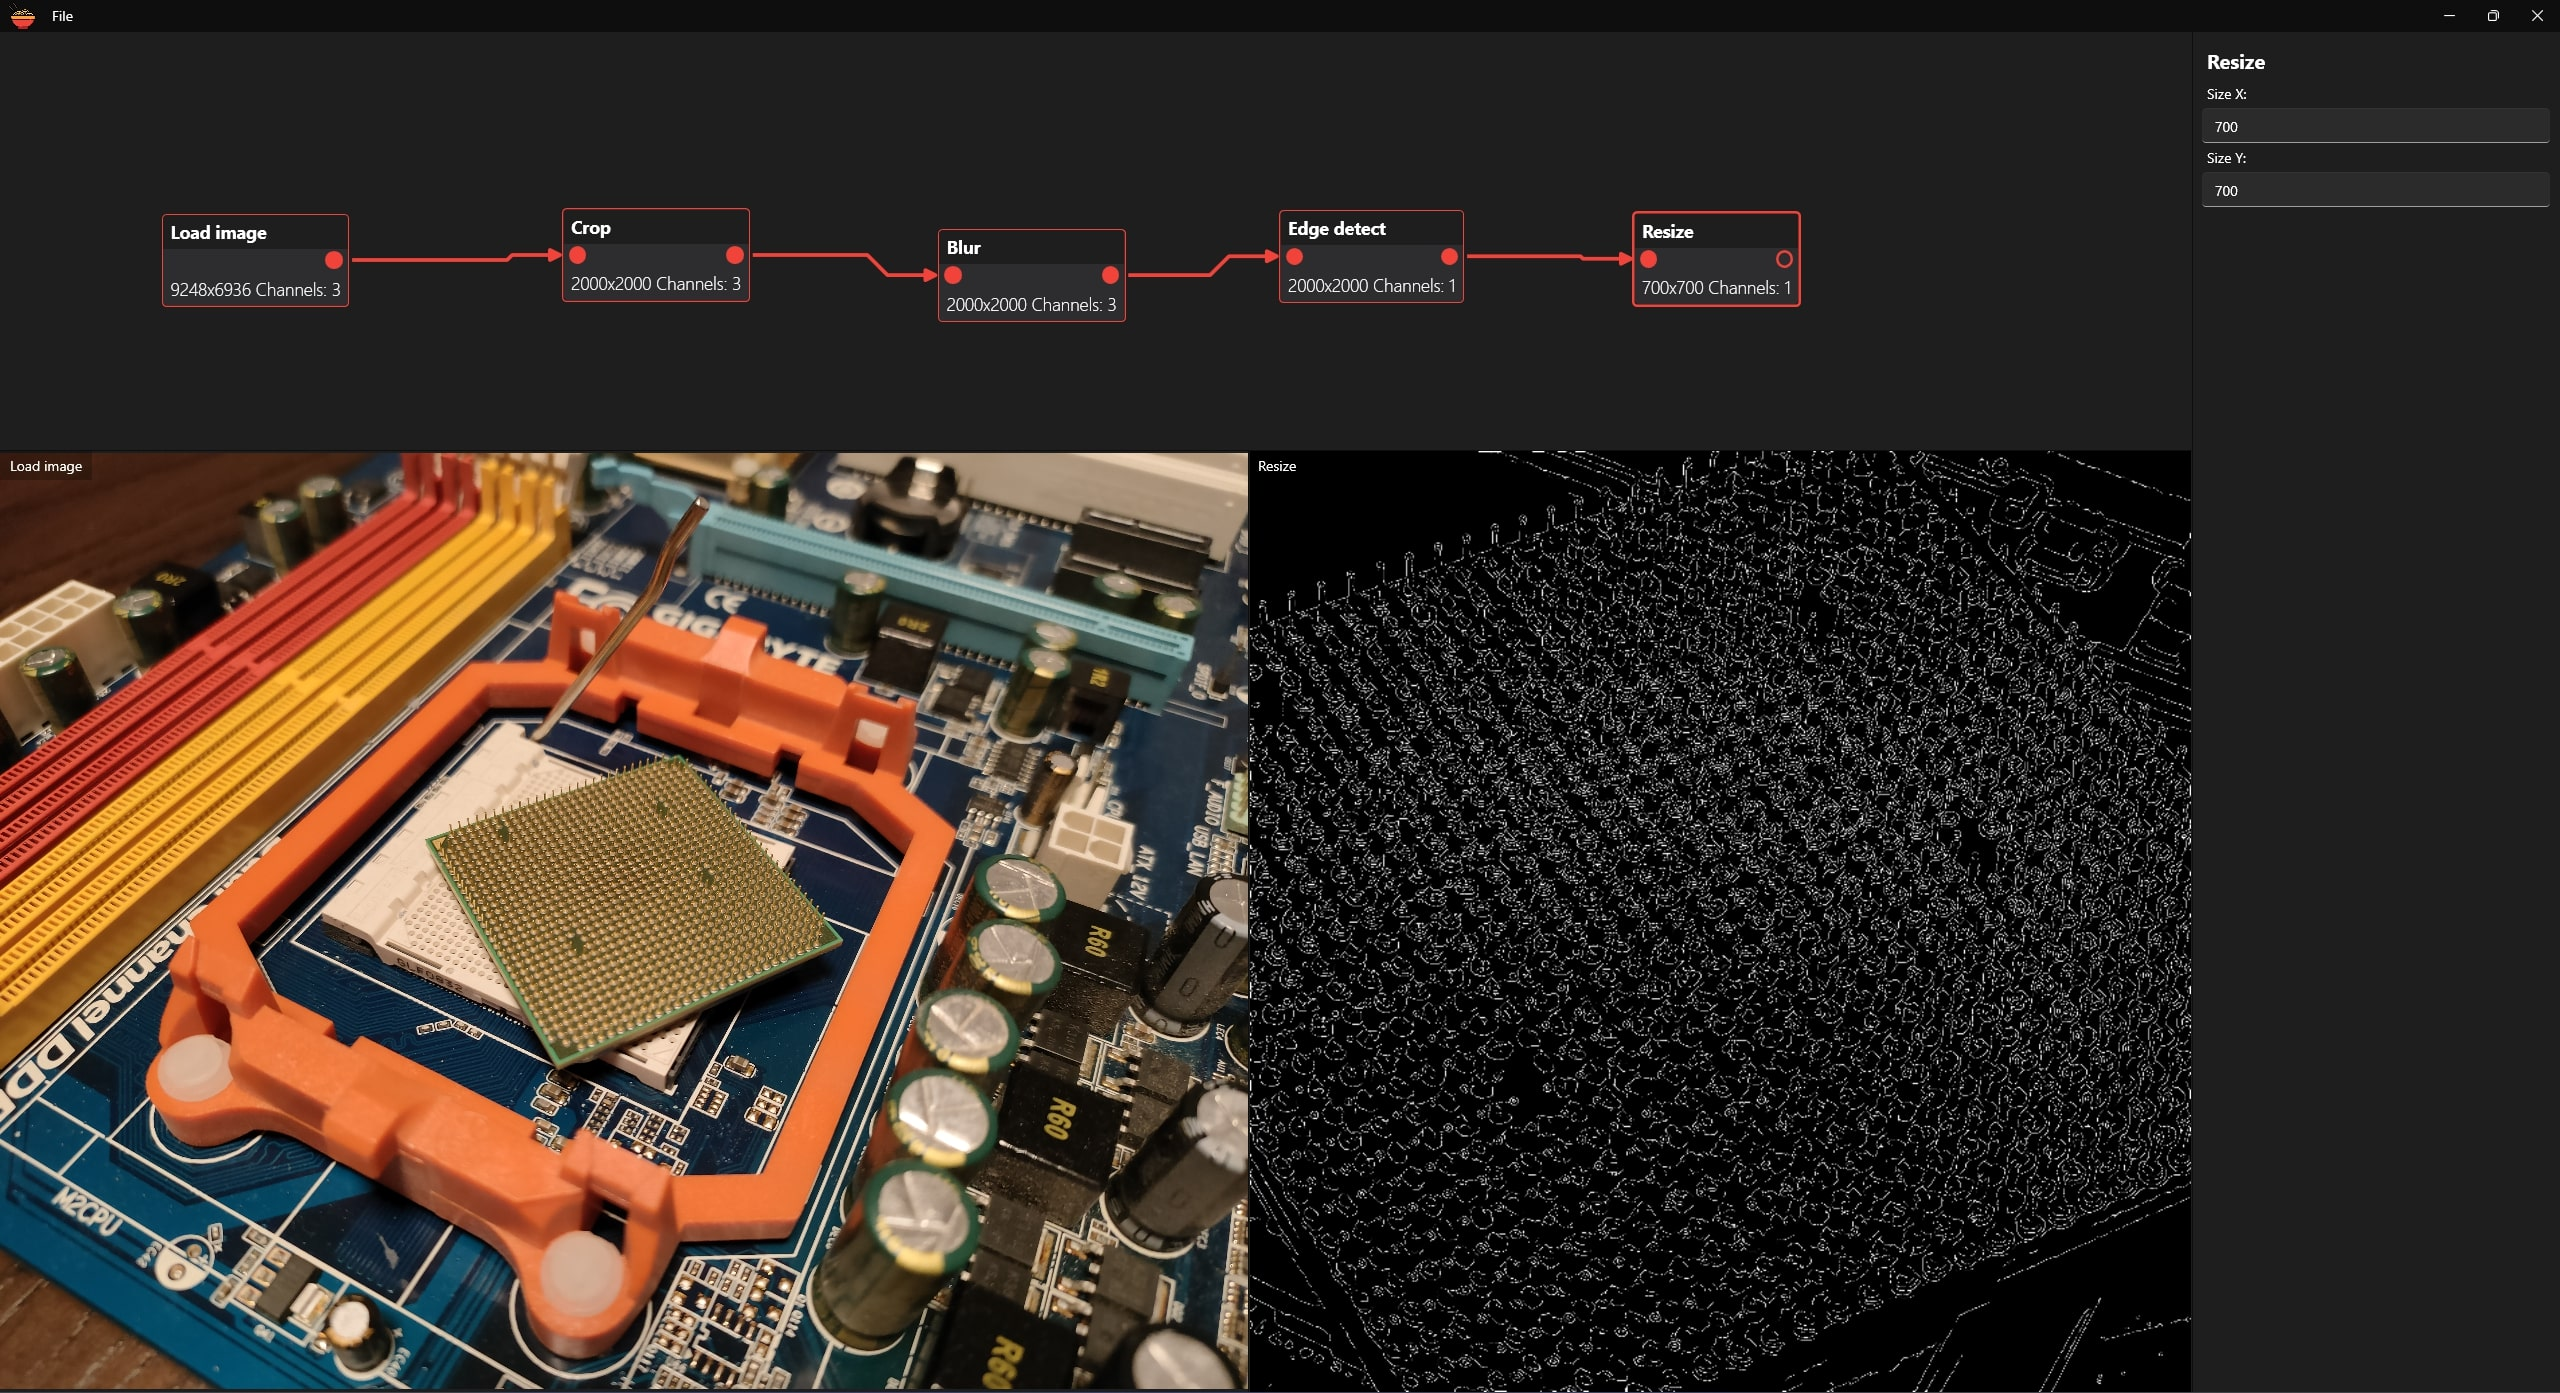
\includegraphics[width=1\linewidth]{images/Picture27.jpg}
    \caption{Wykrywanie krawędzi na wybranym fragmencie obrazu. Opracowanie własne.}
    \label{fig:socket}
\end{figure} 

\begin{figure}[H]
    \centering
    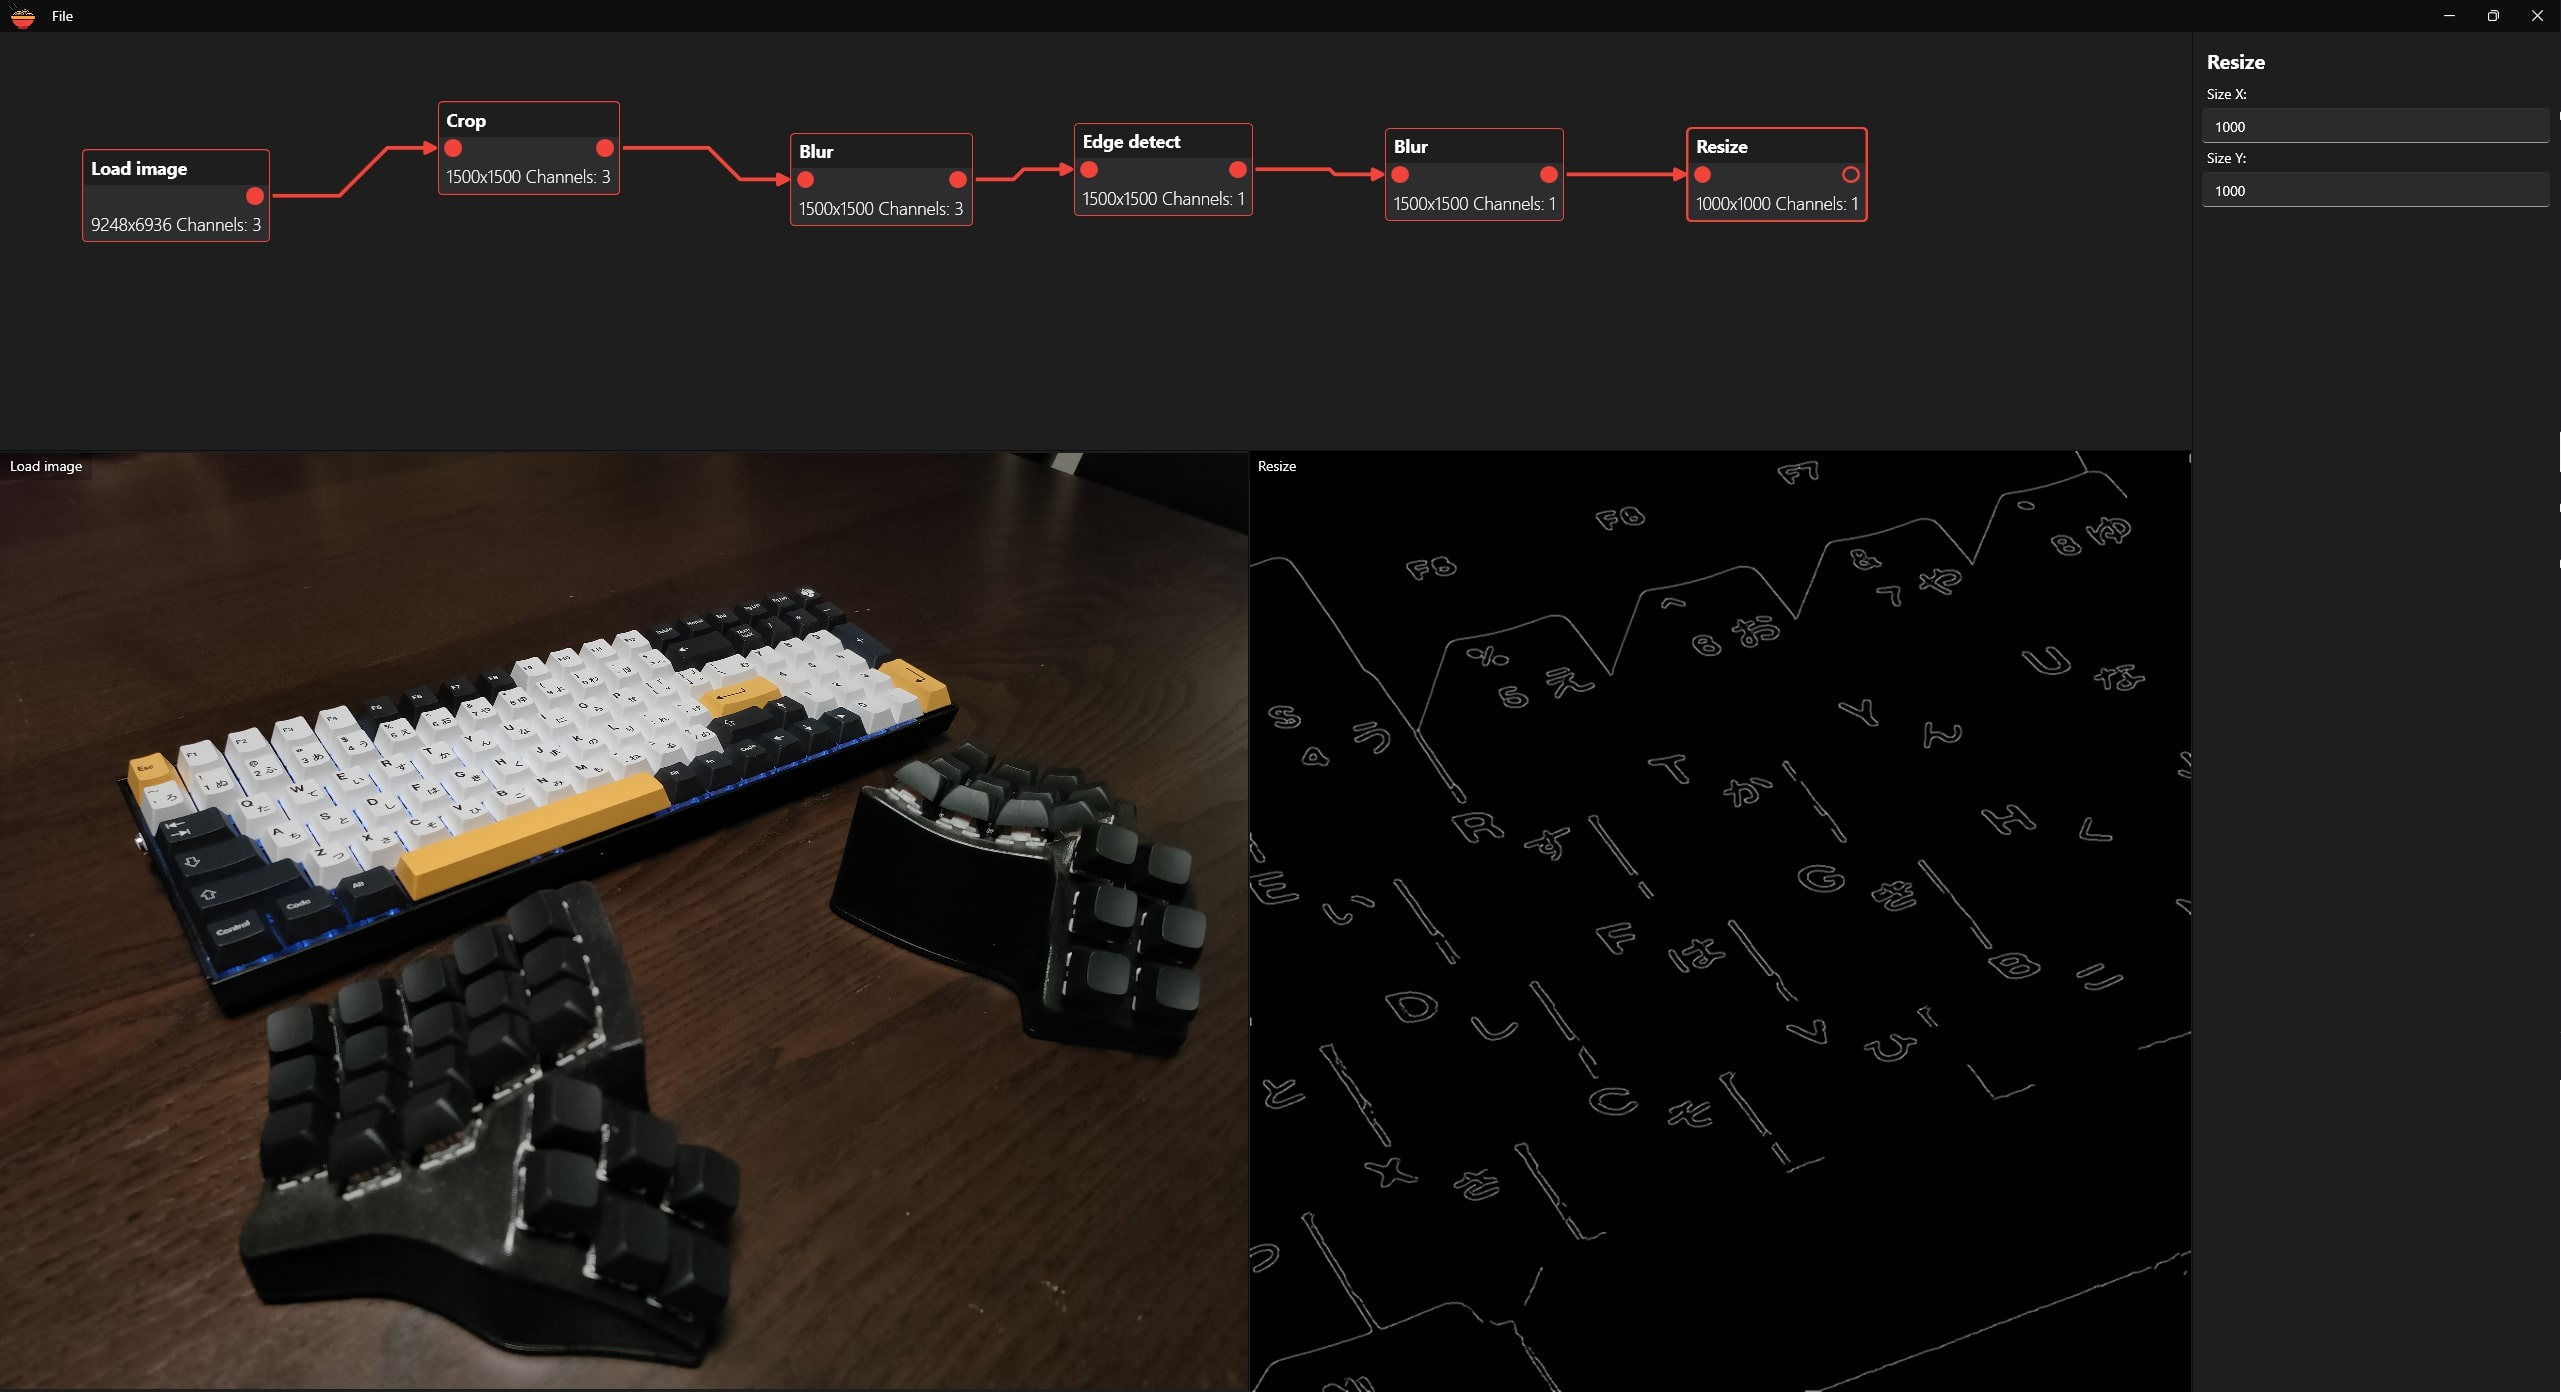
\includegraphics[width=1\linewidth]{images/Picture28.jpg}
    \caption{Wykrywanie krawędzi dla uwydatnienia liter. Opracowanie własne.}
    \label{fig:keyboard}
\end{figure} 

\begin{figure}[H]
    \centering
    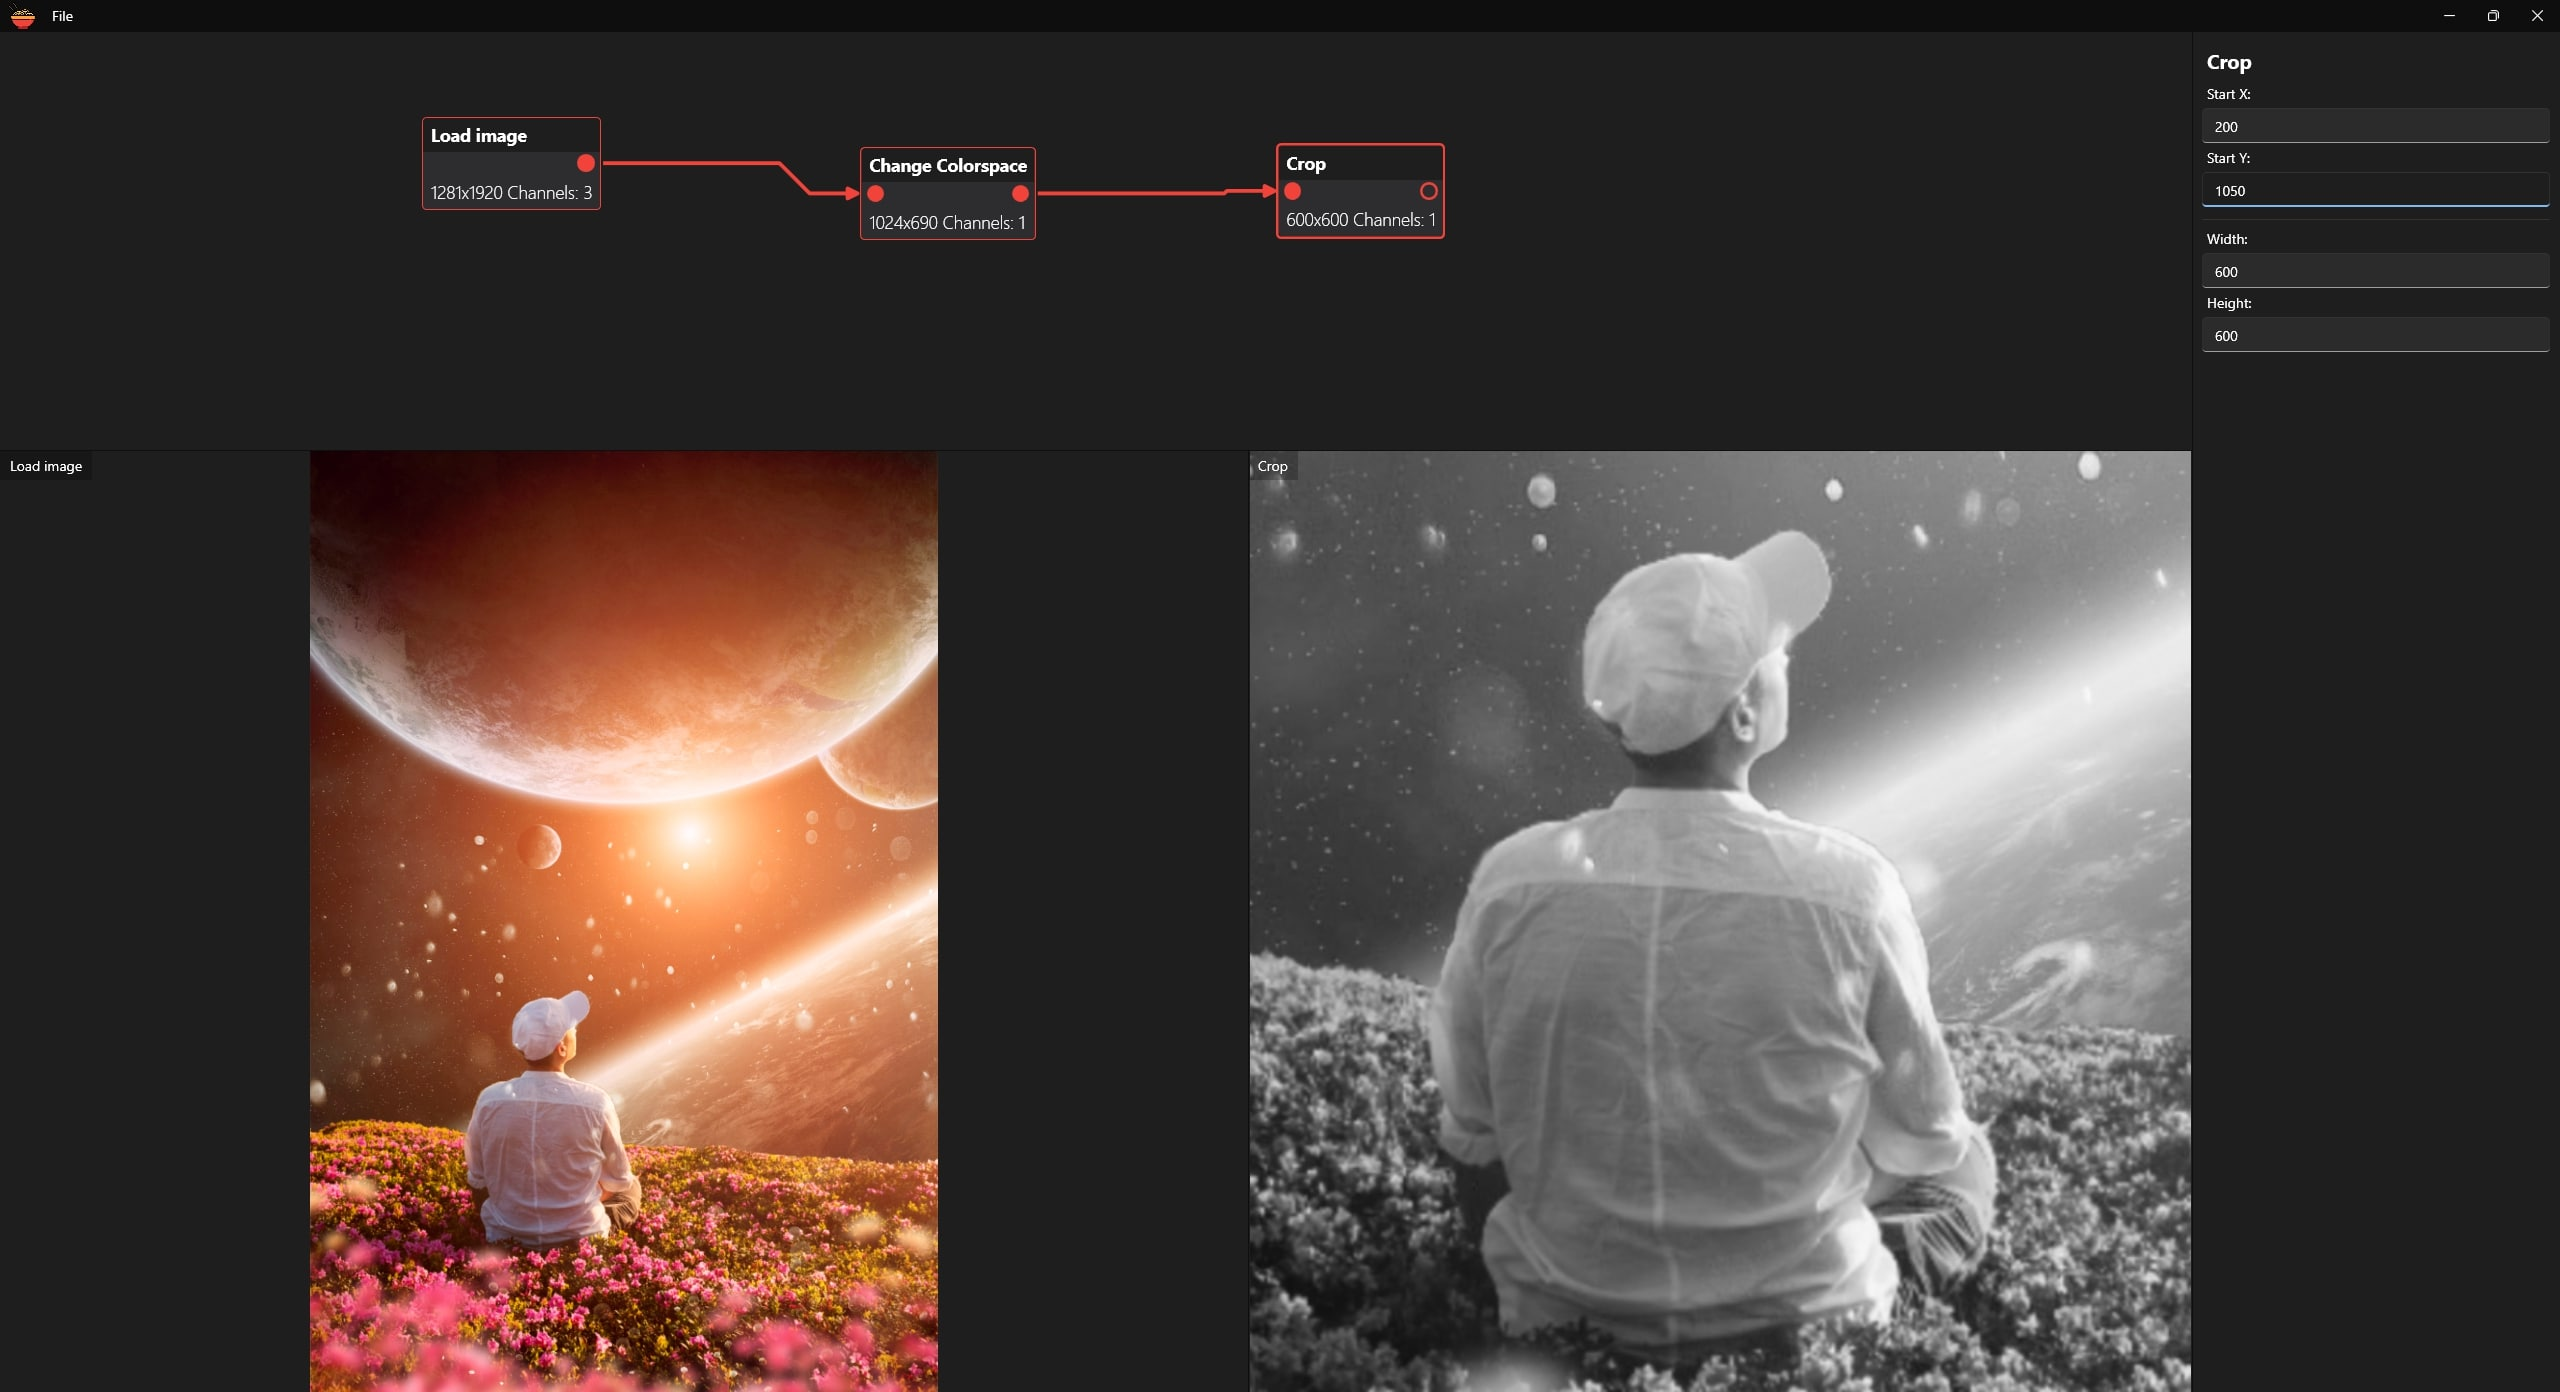
\includegraphics[width=1\linewidth]{images/Picture29.jpg}
    \caption{Obcięcie zdjęcia i zmiana na odcienie szarości. Opracowanie własne.}
    \label{fig:person}
\end{figure} 

\begin{figure}[H]
    \centering
    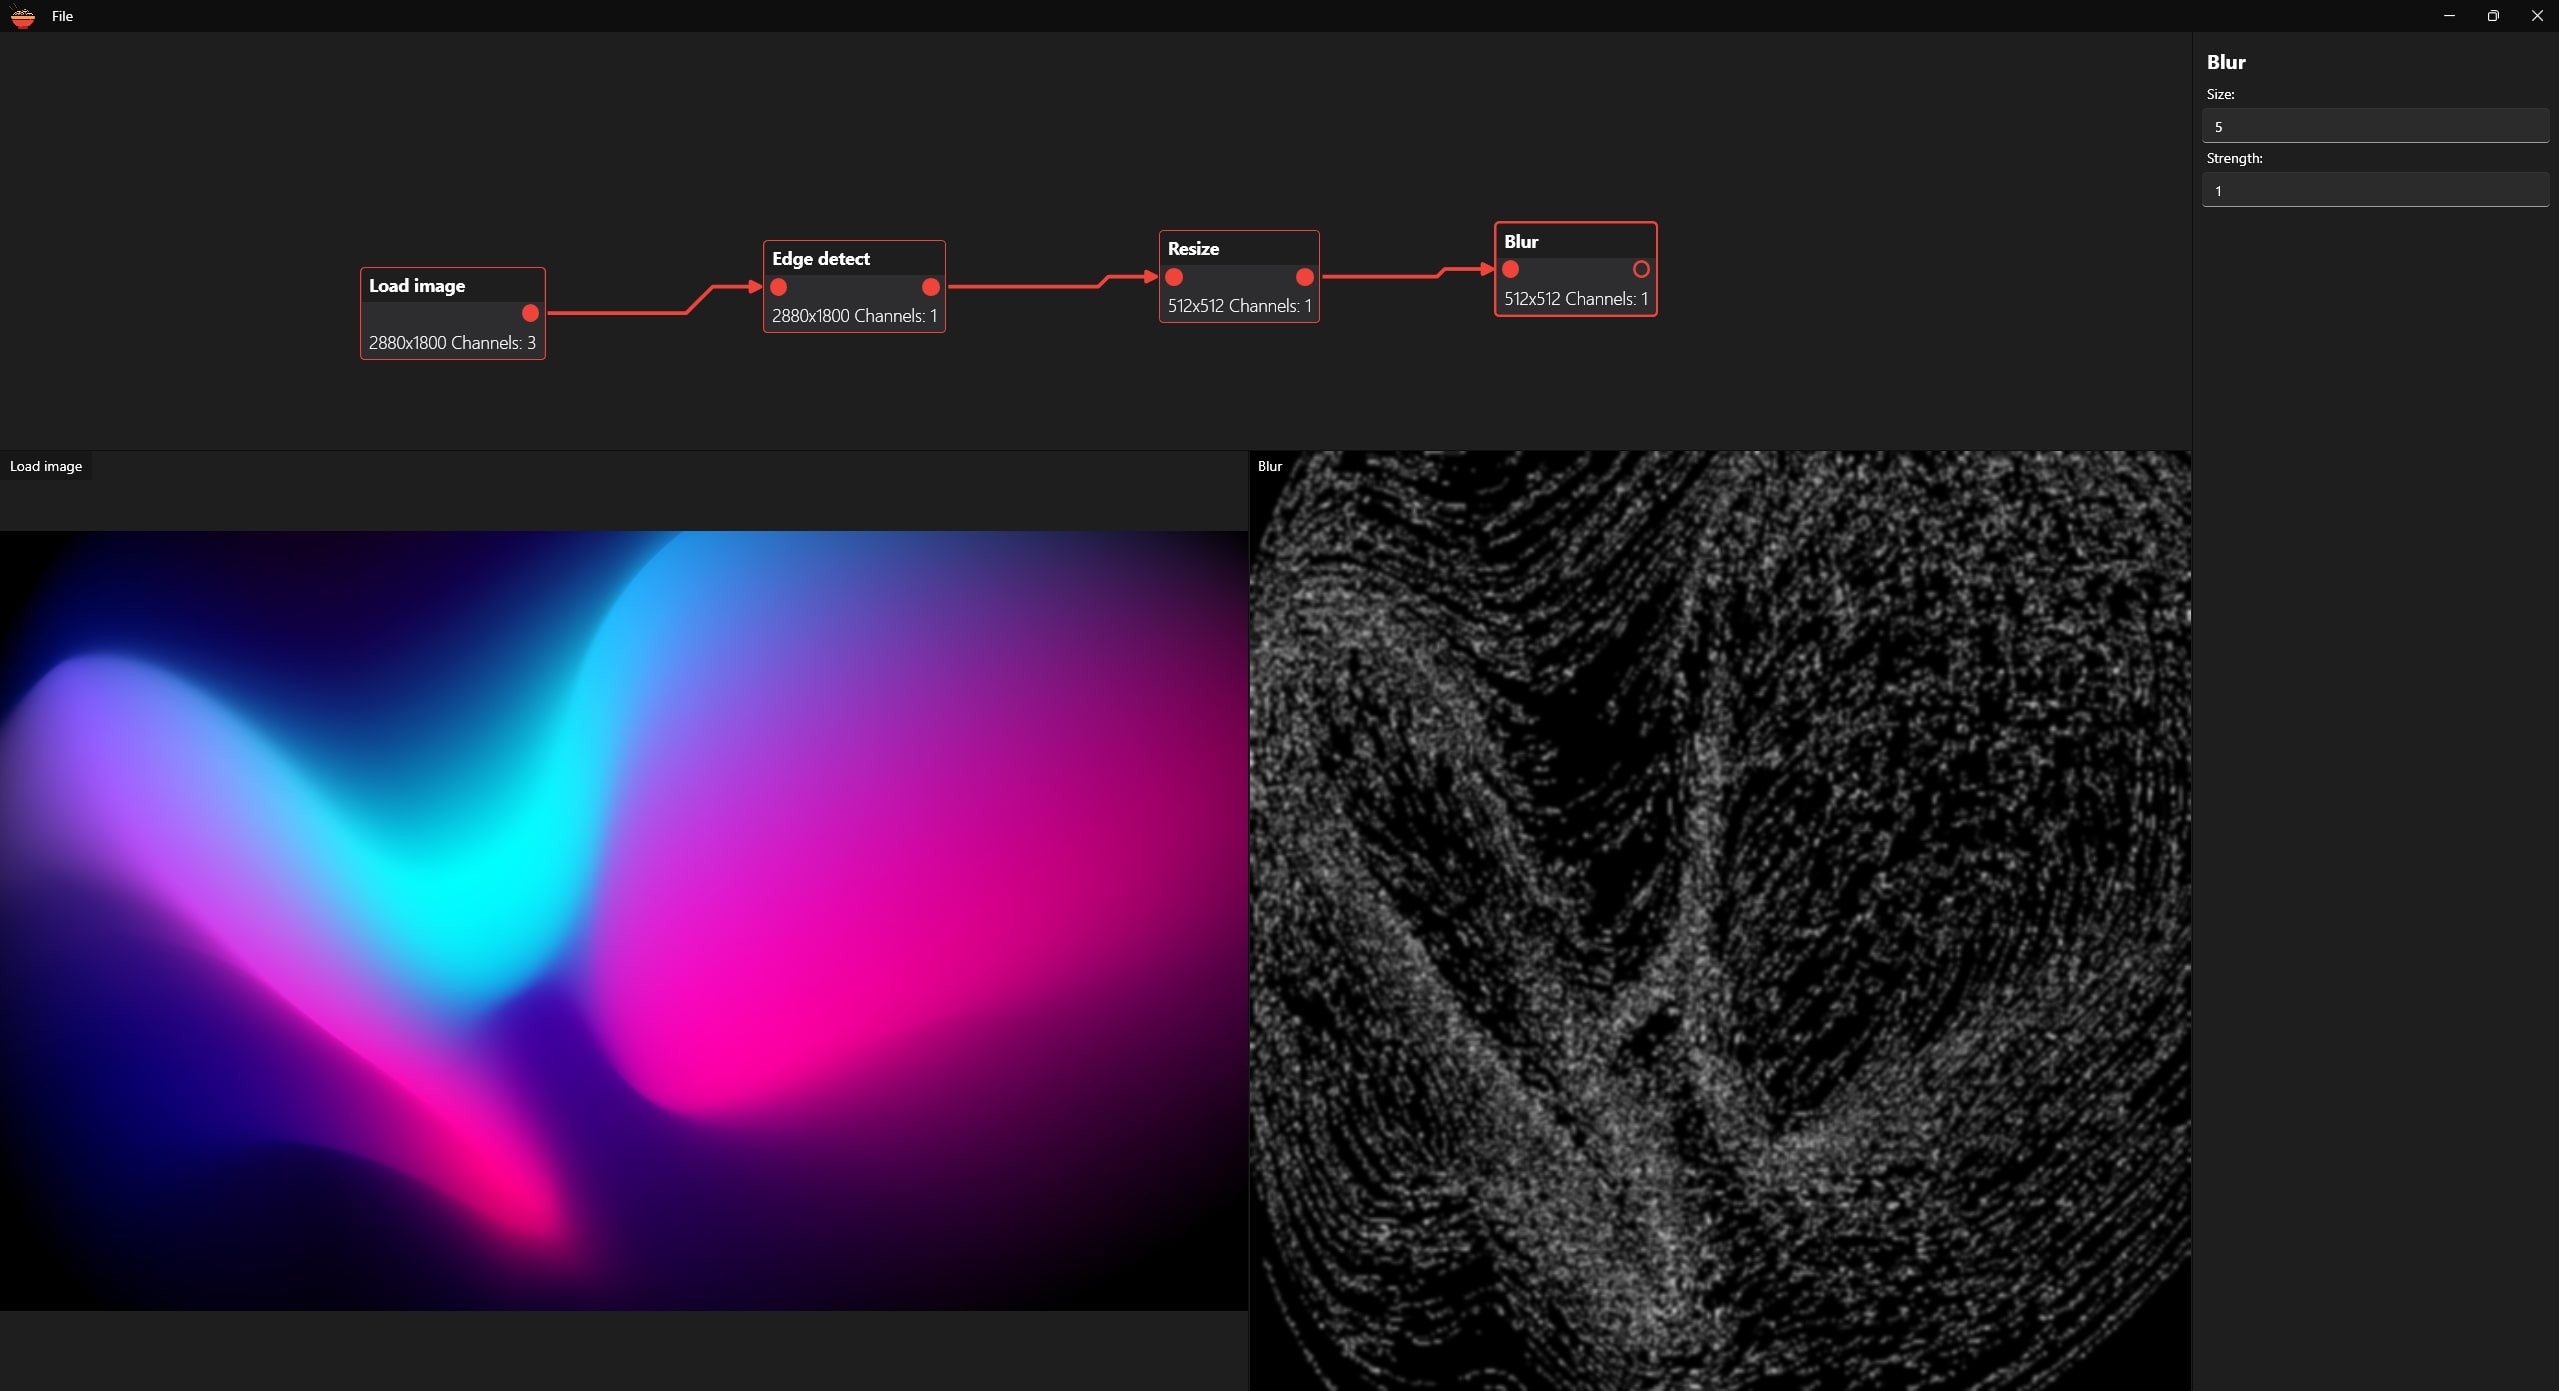
\includegraphics[width=1\linewidth]{images/Picture30.jpg}
    \caption{Abstrakcyjne edytowanie. Opracowanie własne.}
    \label{fig:abstract}
\end{figure} 